%%========================================================================
%% LaTeX sjabloon voor stage/projectrapport of bachelorproef
%%  HoGent Bedrijf en Organisatie
%%========================================================================

%%========================================================================
%% Preamble
%%========================================================================

\documentclass[pdftex,a4paper,12pt,twoside]{report}

% XXX: Let op: dit sjabloon is gemaakt om dubbelzijdig af te drukken
% Voor enkelzijdig, verwijder ``twoside'' hierboven.

%%---------- Extra functionaliteit ---------------------------------------

\usepackage[utf8]{inputenc}  % Accenten gebruiken in tekst (vb. é ipv \'e)
\usepackage{amsfonts}        % AMS math packages: extra wiskundige
\usepackage{amsmath}         %   symbolen (o.a. getallen-
\usepackage{amssymb}         %   verzamelingen N, R, Z, Q, etc.)
\usepackage[dutch]{babel}    % Taalinstellingen: woordsplitsingen,
                             %  commando's voor speciale karakters
                             %  ("dutch" voor NL)
\usepackage{eurosym}         % Euro-symbool €
\usepackage{geometry}
\usepackage{graphicx}        % Invoegen van tekeningen
\usepackage[pdftex,bookmarks=true]{hyperref}
                             % PDF krijgt klikbare links & verwijzingen,
                             %  inhoudstafel
\usepackage{listings}        % Broncode mooi opmaken
\usepackage{multirow}        % Tekst over verschillende cellen in tabellen
\usepackage{rotating}        % Tabellen en figuren roteren
\usepackage{natbib}          % Betere bibliografiestijlen
\usepackage{fancyhdr}        % Pagina-opmaak met hoofd- en voettekst

\usepackage[T1]{fontenc}     % Ivm lettertypes
\usepackage{lmodern}
\usepackage{textcomp}
\usepackage{listings}

\usepackage{lipsum}          % Voor vultekst (lorem ipsum)

\usepackage{float}
\usepackage{glossaries}
\usepackage{blindtext}
\usepackage{scrextend}
\addtokomafont{labelinglabel}{\sffamily}
\makenoidxglossaries




%%---------- Layout ------------------------------------------------------

% hoofdingen, enz.
\pagestyle{fancy}
% enkel hoofdstuktitel in hoofding, geen sectietitel (vermijd overlap)
\renewcommand{\sectionmark}[1]{}

% lijn, wordt gebruikt in titelpagina
\newcommand{\HRule}{\rule{\linewidth}{0.5mm}}

% Leeg blad
\newcommand{\emptypage}{
\newpage
\thispagestyle{empty}
\mbox{}
\newpage
}

% Gebruik een schreefloos lettertype ipv het "oubollig" uitziende
% Computer Modern
\renewcommand{\familydefault}{\sfdefault}

% Commando voor invoegen Java-broncodebestanden (dank aan Niels Corneille)
% Gebruik: \codefragment{source/MijnKlasse.java}{Uitleg bij de code}
\newcommand{\codefragment}[2]{ \lstset{%
  language=java,
  breaklines=true,
  float=th,
  caption={#2},
  basicstyle=\scriptsize,
  frame=single,
  extendedchars=\true
}
\lstinputlisting{#1}}

%%---------- Documenteigenschappen ---------------------------------------
%% Vul dit aan met je eigen info:

% Je eigen naam
\newcommand{\student}{Tim Van Roosbroeck}

% De naam van je lector, begeleider, promotor
\newcommand{\promotor}{Sebastiaan Labijn}

% De naam van je co-promotor
\newcommand{\copromotor}{Joeri Van Steen}

% Indien je bachelorproef in opdracht van een bedrijf of organisatie
% geschreven is, geef je hier de naam.
\newcommand{\instelling}{---}

% De titel van het rapport/bachelorproef
\newcommand{\titel}{Adblocker en de impact op gratis content beschikbaar op het internet.}

% Datum van indienen
\newcommand{\datum}{29 mei 2016}

% Faculteit
\newcommand{\faculteit}{Faculteit Bedrijf en Organisatie}

% Soort rapport
\newcommand{\rapporttype}{Scriptie voorgedragen tot het bekomen van de graad van\\Bachelor in de toegepaste informatica}

% Academiejaar
\newcommand{\academiejaar}{2015-2016}

% Examenperiode
%  - 1e semester = 1e examenperiode
%  - 2e semester = 2e examenperiode
%  - tweede zit = 3e examenperiode
\newcommand{\examenperiode}{Tweede examenperiode}

%%========================================================================
%% Inhoud document
%%========================================================================

\begin{document}
%%---------- Front matter ------------------------------------------------
%% Het voorblad - Hier moet je in principe niets wijzigen.

\begin{titlepage}
\newgeometry{top=2cm,bottom=1.5cm,left=1.5cm,right=1.5cm}
  \begin{center}

    \begingroup
    \rmfamily
    
\includegraphics[width=2.5cm]{img/HG-beeldmerk-woordmerk}\\[.5cm]
    \faculteit\\[3cm]
    \titel
    \vfill
    \student\\[3.5cm]
    \rapporttype\\[2cm]
    Promotor:\\
    \promotor\\
    Co-promotor:\\
    \copromotor\\[2.5cm]
    
    Academiejaar: \academiejaar\\[.5cm]
    \examenperiode
    \endgroup

  \end{center}
  \restoregeometry
\end{titlepage}


% Schutblad

\emptypage


\begin{titlepage}
  \newgeometry{top=5.35cm,bottom=1.5cm,left=1.5cm,right=1.5cm}
  \begin{center}

    \begingroup
    \rmfamily
    \faculteit\\[3cm]
    \titel
    \vfill
    \student\\[3.5cm]
    \rapporttype\\[2cm]
    Promotor:\\
    \promotor\\
    Co-promotor:\\
    \copromotor\\[2.5cm]
    
    Academiejaar: \academiejaar\\[.5cm]
    \examenperiode
    \endgroup

  \end{center}
  \restoregeometry
\end{titlepage}


\begin{abstract}

Het doel van deze studie is een onderzoek naar de huidige en toekomstige impact van het gebruik van ad blockers.
Hiervoor heb ik nagegaan welke de evolutie is van advertenties op websites en de relatie met het ontstaan van ad blockers. Er wordt een beeld geschetst van de verschillende soorten internetadvertenties die gebruikt worden.
Ik ga na welke soort ad blockers er worden gebruikt. Tevens beschrijf ik hoe ze werken en op welke manier de bedrijven erachter hun inkomsten verwerven.
Een gebruikersonderzoek geeft ons aan welke de redenen zijn voor het activeren van advertentieblokkering. Deze studie geeft ons ook inzage in de verschillende gebruikerstypes. De spreiding wordt demografisch, geografisch, over de verschillende browsers en soorten inhoud in kaart gebracht. Ook de vraag in welke mate de gebruiker bereid is om voor inhoud te betalen, werd gesteld.
De economische gevolgen van het gebruik van advertentieblokkering voor de verschillende betrokken partijen worden becijferd zowel wereldwijd als Europees en lokaal. Tevens heb ik onderzocht welke evolutie te verwachten is op korte en lange termijn.
Ik heb bekeken hoe de inhoud-aanbieders en de adverteerders zich wapenen tegen het gebruik van ad blockers. Dit wordt zowel technologisch aangepakt als door zoeken naar andere manieren van adverteren. 
Ik heb nagegaan of de technologieën die gebruikt worden om advertentieblokkering te detecteren niet in strijd zijn met bestaande wetgeving.
Tot slot geef ik aan op welke manier alle betrokken partijen op zoek gaan naar een evenwicht tussen de kost van inhoudsverstrekking, inkomsten en gebruikerservaring. 



\end{abstract}

\chapter*{Voorwoord}
\label{ch:voorwoord}

% TODO: Vergeet ook niet te bedanken wie je geholpen/gesteund/... heeft
Dit document is het resultaat van de opdracht tot het schrijven van een bachelorproef om mijn opleiding bachelor in de toegepaste informatica af te ronden. Een aantal personen heeft mij geholpen dit te verwezenlijken en die mensen zou ik via deze weg graag bedanken. 

De eerste persoon is mijn promotor Sebastiaan Labijn de mij gedurende het schrijven van deze scriptie veel heeft geholpen door het geven van tips en nuttige feedback. 

Als tweede wil ik graag mijn co-promotor Joeri Van Steen bedanken. Hij stond altijd klaar om mijn inhoudelijke vragen te beantwoorden. 

Als laatste wil ik alle personen bedanken die mij hebben bijgestaan met spelling en zinsconstructie, in het bijzonder mijn ouders.



\tableofcontents


%\newglossaryentry{tracker}
%{
  %name=tracker,
  %description={Een soort van cookie waarbij een logboek van de online activiteiten van een gebruiker worden gekoppeld aan zijn Internet Protocol(IP) adres. De tracker stuurt deze informatie door naar een externe database voor analyse. Samen met gegevens van miljoenen anderen worden die gegevens dan gebruikt voor bijvoorbeeld marketing analyse. Deze tracker blijft werken ook al heeft men de site waar de tracker gedownload werd  al lang verlaten.  },
	%plural={trackers}
%}
%\newglossaryentry{cross-site request}
%{
  %name=cross-site request,
  %description={Een cross-site request is een request naar een volledig andere webpagina, die de browser in opdracht van een webpagina uitvoerd. },
	%plural={cross-site requests}
%}
%\newglossaryentry{Affiliate marketing}
%{
  %name={Affiliate marketing},
  %description={
	%Affiliate marketing is een vorm van internetmarketing waarbij adverteerders hun partners (affiliates) belonen voor de gegenereerde verkopen of leads (zoals lidmaatschappen - abonnementen) die de affiliate heeft aangeleverd. Affiliates kunnen dit bewerkstelligen door onder andere advertenties van adverteerders op hun website te plaatsen. Als er uit het doorverwijzen van klanten naar de adverteerders een verkoop of lead volgt, ontvangt de affiliate hiervoor een vergoeding van de adverteerder. },
	%plural={Affiliate marketing}
%}
%
%\newglossaryentry{css selectors}
%{
  %name=css selector,
  %description={In css worden selectors gebruikt om te selecteren welke delen moeten gebruik maken van een bepaalde stijl.},
	%plural={css selectors}
%}
%\newglossaryentry{whitelist}
%{
  %name={whitelist},
  %description={Een whitelist van een ad blocker is een lijst met webpagina's waarop de ad blocker uitgeschakeld zal zijn en waarbij advertenties wel getoond zullen worden.},
	%plural={whitelist}
%}

%\glsaddall
%\printnoidxglossaries
\newpage 
\begin{labeling}{alligator}

\item [\textbf{Affiliate marketing}] Dit is een vorm van internetmarketing waarbij adverteerders hun partners (affiliates) belonen voor de gegenereerde verkopen of leads (zoals lidmaatschappen - abonnementen) die de affiliate heeft aangeleverd. Affiliates kunnen dit bewerkstelligen door onder andere advertenties van adverteerders op hun website te plaatsen. Als er uit het doorverwijzen van klanten naar de adverteerders een verkoop of lead volgt, ontvangt de affiliate hiervoor een vergoeding van de adverteerder.


\item [\textbf{blog}] Een blog is een soort van dagboek op het internet.

\item [\textbf{cross-site request}] Een cross-site request stuurt bezoekers door naar een volledig andere website, die de browser in opdracht van een webpagina uitvoert.

\item [\textbf{css}] Cascading style sheets zorgen voor de lay-out van een webpagina.

\item [\textbf{e-commerce}] Elektronische bedrijfsvoering is de verzameling van alle manieren waarop op het internet aan handel wordt gedaan.

\item [\textbf{ePrivacy directive}] De ePrivacy directive is een Europese richtlijn voor digitale gegevensbescherming.

\item [\textbf{extensie}] Extensies zijn software die extra functionaliteiten toevoegen aan een computerprogramma. 

\item [\textbf{HTML DOM}] Het HTML document object model is de boomstructuur van HTML elementen die zich op een webpagina bevinden.

\item [\textbf{IAB}] Het Internet Advertising Bureau is een organisatie die de belangen verdedigt van adverteerders en uitgevers.

\item [\textbf{malware}] Malware is de naam voor software die gemaakt is om computersystemen te beschadigen, of om toegang te krijgen tot die computersystemen zonder toestemming van de gebruiker.

\item [\textbf{ppc}] Pay per click of betaal per klik is een advertentiemodel waarbij adverteerders slechts betaald worden als er op de advertentie geklikt wordt. Het is dus niet voldoende dat bezoekers de advertentie zien.

\item [\textbf{pre-roll}] Een pre-roll is een advertentievideo die wordt afgespeeld vóór de video die een bezoeker van een website echt wil bekijken.


\item [\textbf{reguliere expressies}] Een reguliere expressie is een reeks van karakters die een zoekpatroon bepalen. Ze bieden een simpele en efficiënte manier om tekst te doorzoeken.

\item [\textbf{tracker}] Een soort cookie waarbij een logboek van de online activiteiten van een gebruiker worden gekoppeld aan zijn Internet Protocol(IP) adres. De tracker stuurt deze informatie door naar een externe database voor analyse. Samen met gegevens van miljoenen anderen worden die gegevens dan gebruikt voor bijvoorbeeld marketing analyse. Deze tracker blijft doorwerken ook al heeft men de site waar de tracker gedownload werd  al lang verlaten.

\item [\textbf{whitelist}] Een whitelist van een ad blocker is een lijst met websites waarop de ad blocker uitgeschakeld zal zijn, waardoor de advertenties wel getoond zullen worden.







%\item [\textbf{whitelist}] Een witte lijst is een opsomming van zaken, in dit geval websites, die toegelaten worden.




\end{labeling}
% Als je een lijst van afkortingen of termen wil toevoegen, dan hoort die
% hier thuis. Gebruik bijvoorbeeld de ``glossaries'' package.

%%---------- Kern --------------------------------------------------------

\chapter{Inleiding}
\label{ch:inleiding}

Samen met de toename in het gebruik van het internet, evolueerde ook het gebruik van dit medium voor publiciteitsdoeleinden. Tijdens de jaren ’90 deed het internet zijn intrede als reclamemedium. Naarmate meer en meer bedrijven het internet gebruiken om hun kennis, kunde en producten voor te stellen, groeit de gedachte om expliciet advertenties op de pagina’s van drukbezochte websites te plaatsen. Webvertising is een feit.
\\
Wat eerst op een schuchtere manier gebeurt, explodeert in de 21ste eeuw. Zowel via email (ook wel spam genaamd) als via webpagina’s worden internetgebruikers bestookt met allerhande reclameboodschappen. De technologie evolueert snel, alsook de manier waarop publiciteit gelinkt wordt aan het surfgedrag. Zoals steeds liggen excessen aan de basis van oppositie. Wat eerst leuk leek, wordt irritant. Opdringerige advertenties behoren tot de grootste ergernissen van internetgebruikers. Enkele banners worden vaak niet als probleem ervaren, maar sommige sites maken het erg bont. Dit verstoord evenwicht ligt wellicht aan de basis van het ontstaan van ad blocker software rond 2006.

% De inleiding moet de lezer alle nodige informatie verschaffen om het onderwerp te begrijpen zonder nog externe werken te moeten raadplegen \citep{Pollefliet2011}. Dit is een doorlopende tekst die gebaseerd is op al wat je over het onderwerp gelezen hebt (literatuuronderzoek).

% Je verwijst bij elke bewering die je doet, vakterm die je introduceert, enz. naar je bronnen. In \LaTeX{} kan dat met het commando \texttt{$\backslash${cite\{\}}} of \texttt{$\backslash${citep\{\}}}. Als argument van het commando geef je de ``sleutel'' van een ``record'' in een bibliografische databank in het Bib\TeX{}-formaat (een tekstbestand). Als je expliciet naar de auteur verwijst in de zin, gebruik je \texttt{$\backslash${}cite\{\}}.
% Soms wil je de auteur niet expliciet vernoemen, dan gebruik je \texttt{$\backslash${}citep\{\}}. Hieronder een voorbeeld van elk.

% \cite{Knuth1998} schreef een van de standaardwerken over sorteer- en zoekalgoritmen. Experten zijn het erover eens dat cloud computing een interessante opportuniteit vormen, zowel voor gebruikers als voor dienstverleners op vlak van informatietechnologie~\citep{Creeger2009}.

\section{Probleemstelling en Onderzoeksvragen}
\label{sec:onderzoeksvragen}

Het doel van dit onderzoek is inzicht te krijgen in de werking van ad blockers. Daarnaast wordt bekeken wat de impact van het gebruik van ad blocking is op korte en op lange termijn. Hoe reageren de bedrijven die hun inkomsten uit reclame dreigen te verliezen?

%Het doel van het onderzoek is enerzijds inzicht te krijgen in de werking van adblockers en anderzijds het bepalen van de impact en de gevolgen op korte en lange termijn op de bedrijven die hun inkomsten halen uit reclame, en wat die bedrijven hun reactie is op ad blockers.
\begin{itemize}
	\item Wat is de impact, op dit moment en in de toekomst, van ad blockers op reclame inkomsten? 
	\item Op welke manieren omzeilen content providers momenteel ad blockers? Hoe zullen ze zich in de toekomst wapenen tegen ad blockers?
\end{itemize}

% TODO: Wees zo concreet mogelijk bij het formuleren van je
% onderzoeksvra(a)g(en). Een onderzoeksvraag is trouwens iets waar nog
% niemand op dit moment een antwoord heeft (voor zover je kan nagaan).


\chapter{Methodologie}
\label{ch:methodologie}
\section{Internet en publiciteit}
In het eerste hoofdstuk wordt er onderzoek gedaan naar publiciteit op het internet. De evolutie van reclame wordt onderzocht om het ontstaan van ad blockers beter te begrijpen. Om in een later hoofdstuk de redenen van gebruik van ad blockers te bepalen worden de soorten reclame onderzocht. Om later de impact op korte en lange termijn beter te begrijpen wordt hier onderzoek gedaan naar reclamenetwerken en de inkomsten uit advertenties.
\section{De ad blockers}
In dit hoofdstuk wordt de werking van ad blockers verduidelijkt. Hier wordt ook bepaald welke verschillende ad blockers er zijn en wat hun business model is.
\section{Evolutie gebruik ad blockers}
Om de impact van ad blockers in een later hoofdstuk te bepalen wordt er in dit hoofdstuk gekeken naar de groei, de spreiding en de redenen voor gebruik van ad blockers.
\subsection{Laadsnelheid van ad blockers}
Om een idee te krijgen of er impact is op de laadsnelheid van internet pagina’s door het gebruik van ad blockers, heb ik zelf onderstaande proefneming uitgevoerd.
\\
Opstelling:
\begin{itemize}
	\item Browser: Chrome.
	\item Add-on voor de testen: Apptelemetry.
	\item Besturingssysteem: Windows 8.1.
	\item Ad blocker: Adblock Plus.
\end{itemize}
De pagina test wordt op volgende manier uitgevoerd:
\begin{enumerate}
	\item Start browser (zonder adblocker).
	\item Voer de URL in.
	\item Noteer de Apptelemetry meetresultaten.
	\item De cache leegmaken.
	\item Browser sluiten.
\end{enumerate}

Deze stappen worden voor elke website 10 maal uitgevoerd. Hetzelfde testscenario wordt tevens uitgevoerd met de ad blocker geactiveerd. Voor de resultaten zie hoofdstuk \ref{sec Laadsnelheid en bandbreedte}.

\section{Impact van ad blockers}
In dit hoofdstuk bepalen we de impact op de verschillende partijen. De resultaten uit voorgaande hoofdstukken worden in dit hoofdstuk gebruikt om de impact van ad blockers te onderzoeken. Daarnaast wordt de impact op websites verder onderzocht door interviews met internet-inhoudsaanbieders.
\subsection{Interviews met internet-inhoudsaanbieders}
Om hierover meer te weten te komen zocht ik contact op met 15 internet-inhoudsaanbieders. Daarvan bleven uiteindelijk drie personen over die ik telefonisch of via Skype contacteerde.
\\
Contactpersonen:
\begin{itemize}
	\item Peter Soetens: directeur digitale nieuwsmedia van Mediahuis nv.
	\item Brad Overbey: een YouTuber genaamd Drift0r met een focus op videospellen.
	\item Jerry Berg: een YouTuber genaamd Barnacules Nerdgasm met een focus op technische videos.
\end{itemize}

Voor de resultaten van de interviews zie hoofdstuk \ref{sec:Impact op de webpagina's}. 
\section{Hoe wapenen bedrijven zich tegen ad blockers}
In dit hoofdstuk worden de verschillende manieren onderzocht waarop internet-inhoudsaanbieders de verliezen aan inkomsten door ad blockers kunnen compenseren. Naast methodes om ad blockers tegen te gaan wordt er ook gekeken naar alternatieve inkomstenbronnen.  
\section{Wetgeving en rechtszaken rond ad blockers}
In dit hoofdstuk onderzoeken we hoe de wet tegenover ad blocking staat om te bepalen of internet-inhoudsaanbieders de ontwikkelaars van ad blockers kunnen aanklagen.
% TODO: Hoe ben je te werk gegaan? Verdeel je onderzoek in grote fasen, en
% licht in elke fase toe welke stappen je gevolgd hebt. Verantwoord waarom je
% op deze manier te werk gegaan bent. Je moet kunnen aantonen dat je de best
% mogelijke manier toegepast hebt om een antwoord te vinden op de
% onderzoeksvraag.
\chapter{Internet en publiciteit}
\label{ch:Internet en publiciteit}

\section{Evolutie van reclame}
\label{sec:Evolutie van reclame}
Online adverteren of online marketing is een vorm van reclame die het internet gebruikt om zijn marketing boodschap over te brengen aan de consument. Sinds haar eerste verschijning in de vroege jaren negentig, is de groei van reclame op het internet exponentieel toegenomen. Online adverteren omvat zoekrobot adverteren, sociale media reclame, scherm reclame zoals banners en mobiele reclame. Online adverteren is aanwezig in alle bedrijfstakken die zich op het internet bevinden.
\\
In 1994, toen men nog moest inbellen om connectie te maken tot het internet, verscheen op het eerste online magazine genaamd Hotwire, een schijnbaar onschuldige afbeelding. Dit statisch beeld was waarschijnlijk de eerste advertentie in zijn soort op het internet. Gebruikers die op de afbeelding klikten werden rechtstreeks doorverwezen naar de site van de adverteerder. Deze banneradvertentie toonde de interactiviteit van het internet waar traditionele, éénrichtingsmedia zoals tv, radio en kranten te kort schoten. Adverteerders sprongen snel op de kar van online reclame en in 1999 bereikte de globale advertentie-uitgaven de piek van een miljard dollar.
\begin{figure}[h!]
\centering

\includegraphics[width=12cm]{img/firstbanner}
\caption{De eerste reclamebanner. (thefirstbannerad.com)}
\label{fig: Banner-Ads}
\end{figure}
Naarmate het aantal gebruikers steeg op het internet, groeide het uit tot een goed verkoopmedium. Bedrijven begonnen te investeren in e-commerce en content sites (in eerste instantie online versies van kranten en tijdschriften) en de verkoop van advertentieruimte op deze sites. Naarmate men het internet voor meer activiteiten, zoals winkelen en entertainment gebruikte, werden de tactieken van adverteerders meer gevarieerd. Statische banners maakten plaats voor geanimeerde banners. Daarna kwamen de pop-ups en de pop-under advertenties, gevolgd door de pre-roll video en misschien het belangrijkst de zoek advertentie. 
\\
Naarmate de gebruikers het internet ontdekten als bron voor informatie over producten, winkels en promoties, startte Google met de verkoop van advertentieruimte op basis van zoekopdrachten van de consument. Het Google AdWords Programma liet bedrijven toe om zichzelf aan de consument te tonen op de exacte momenten wanneer gebruikers naar hen, hun diensten of hun producten, op zoek waren. Adverteerders hadden nu de mogelijkheid om minder geld te verspillen aan consumenten die niet ontvankelijk zijn voor hun producten of diensten.
\\
Doordat zowel bedrijven als consumenten in grote getallen naar het internet kwamen voor alle vormen van entertainment en informatie, vergrootte de complexiteit van het web enorm. Wat vroeger een eenvoudige samenwerking was tussen de adverteerders en de inhoud-aanbieders van websites begon alsmaar ingewikkelder te worden door de mogelijkheden die de adverteerders nodig hadden om dichter bij hun doelpubliek te komen. Hieruit zijn de reclame netwerken gegroeid, bedrijven die voor een deel van de opbrengst op zoek gaan naar reclame, statistieken bijhouden en die statistieken gebruiken om persoonlijkere reclame te leveren. Bedrijven die gebruik maken van zulke netwerken geven de controle van wat weergegeven wordt op hun website voor een stuk op. Wanneer het netwerk reclame van mindere kwaliteit levert of reclame levert die weinig te maken heeft met de andere inhoud van de webpagina, kan dat de gebruikerservaring verstoren, en dit zonder medeweten van de eigenaar van de website.
\\
Een volgende stap in de evolutie om advertenties bij het juist doelpubliek te brengen was programmatic buying of programmatisch kopen. Dit is het principe van realtime bieden op advertentieruimte om een specifieke advertentie te tonen aan een bepaalde consument en in een specifieke context. Dit wordt op grote schaal mogelijk gemaakt door allerhande algoritmes die het surfgedrag van de consument analyseren, informatie die onder meer afkomstig is van cookies en van big data.
\\
Het is mede door de exponentiële groei sinds de eerste advertenties, en soms slechte kwaliteit van reclame geleverd door de netwerken, dat de eerste ad blockers in 2006 het licht zagen. Daarnaast groeide het wantrouwen van de gebruiker over wat de adverteerders met hun persoonlijke informatie deden. Op die nood aan privacy brachten de ad blockers ook een antwoord.

\section{Soorten reclame}
\label{sec:Soorten reclame}
\subsection{Banner en display advertising }
\label{sec Banner en display advertising }
Banners zijn reclameafbeeldingen die meestal getoond worden aan de randen van een webpagina voornamelijk aan de bovenkant en de zijkant, figuur \ref{fig: Banner-Ads}. Ze zijn vooral te vinden op nieuwswebsites en blogs. Ze zijn gemakkelijk te implementeren en te onderhouden. De advertenties van de banners komen meestal van reclamenetwerken maar kunnen ook door eigenaars van de website beheerd en verkocht worden, zoals men bij een papieren krant doet. De normale banner heeft maar een doorklikpercentage van 0.27\%,\cite{Chaffey2016}, wat laag is. Maar voor veel bedrijven is naamsbekendheid op zich al heel belangrijk. Bij reclameborden langs de weg of bij tv-reclame kan men namelijk ook niet doorklikken en die bestaan ook nog steeds. Door het lage doorklikpercentage wordt de kostprijs van de advertentie niet bepaald aan de hand van het PPC-model maar wel aan de hand van de views. Met banners worden voornamelijk statische afbeeldingen bedoeld. Wanneer er video's of geluidsfragmenten op de plaats van een banner staan spreekt men van display advertising, de overkoepelende term waar statische banners ook onder vallen.
\begin{figure}[h!]
\centering
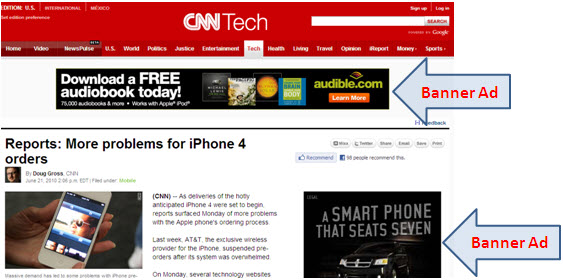
\includegraphics[width=12cm]{img/Banner-Ads}
\caption{Banner ads}
\label{fig: Banner-Ads}
\end{figure}
\subsection{Google search reclame }
\label{sec Google search reclame }
Google Search reclame zijn reclameblokken die getoond worden samen met de zoekresultaten van een Google zoekopdracht, figuur:\ref{fig: Google-Search-ad}. Deze reclame is PPC of Pay per click wat wil zeggen dat de adverteerders betalen per keer dat er op de reclame geklikt wordt. Deze reclame wordt beheerd door het Google’s AdWords platform, dat adverteerders toelaat te bieden op sleutelwoorden. Andere zoekrobotten zoals Bing en Yahoo! hebben een gelijkaardig programma.
\begin{figure}[h!]
\centering
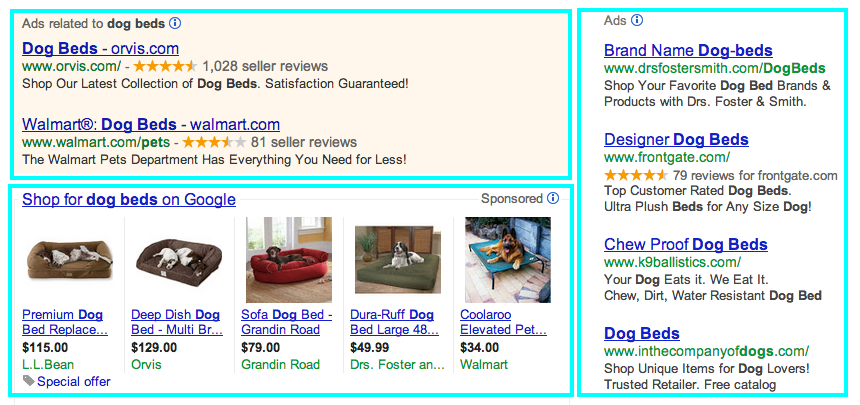
\includegraphics[width=12cm]{img/example-of-google-ads}
\caption{Google search ads}
\label{fig: Google-Search-ad}
\end{figure}
\subsection{Retargeting advertenties }
\label{sec Retargeting advertenties }
Retargeting advertenties houden rekening met de surfgeschiedenis van een gebruiker. Als een gebruiker een website bezoekt zoals Amazon of bol.com kan er een cookie gedownload worden die de gebruiker volgt doorheen zijn surfsessie. Wanneer de gebruiker die site verlaat en andere websites bezoekt, zal die cookie het bezoek aan Amazon of bol.com verzenden naar reclameblokken op die andere websites. De adverteerders kunnen nu reclame maken over het product waar de gebruiker oorspronkelijk op zoek naar was op Amazon, of met behulp van recommendation software gelijkaardige producten aanbieden. Deze vorm van reclame kan door gebruikers ervaren worden als een inbreuk op hun privacy.
\subsection{Sociale media advertenties }
\label{sec Sociale media advertenties }
Sociale media advertenties zijn reclameblokken op sociale netwerkdiensten zoals Facebook, Twitter en Instagram. Eén van de grote voordelen van deze manier van reclame maken is dat adverteerders kunnen profiteren van de grote hoeveelheid informatie die sociale media hebben over hun gebruikers. Adverteerders kunnen daardoor hun advertenties veel efficiënter richten op het juiste doelpubliek.
\section{Reclame netwerken}
\label{sec:Reclamenetwerken}
Een advertentienetwerk is een organisatie die als tussenpersoon dient tussen websites en adverteerders. Een advertentienetwerk zal advertentieruimte van websites verzamelen om deze dan te kunnen aanbieden aan adverteerders. Deze netwerken zijn er gekomen omdat het voor websites moeilijk is om advertenties te verzamelen, en voor adverteerders moeilijk is om advertentie ruimte te vinden voor hun doelpubliek. Naast reclamenetwerken zijn er ook nog ad exchanges. Het verschil is dat men bij netwerken advertentie ruimte koopt, bij exchanges koopt men doelpubliek. Daarnaast werken exchanges via programmatisch kopen, waarbij de adverteerders in realtime bieden op het doelpubliek.


\section{Inkomsten uit reclame}
\label{sec:Inkomsten uit reclame}
Volgens het Internet Advertising Revenu verslag \cite{Silverman2015} van het Interactive Advertising Bureau, IAB, steeg de totale uitgave aan internetreclame in 2014 wereldwijd tot een historisch hoogtepunt van 135 miljard Amerikaanse dollar, met een gemiddelde groei van 17\%.

\begin{figure}[h!]
\centering
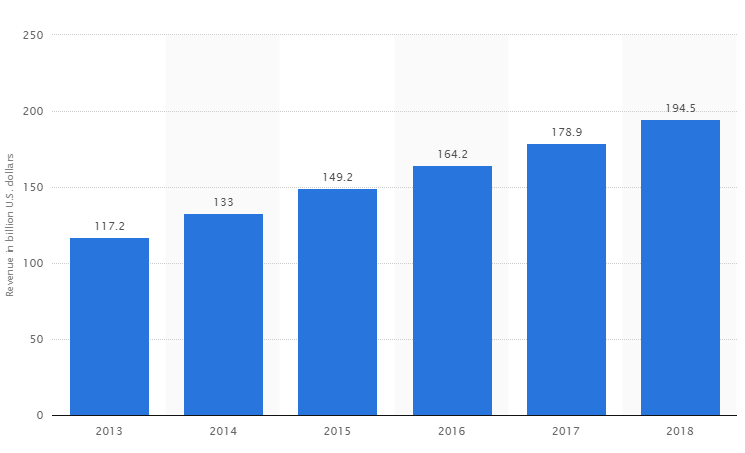
\includegraphics[width=12cm]{img/AdvertisingRevenueYearly}
\caption{ Jaarlijkse uitgaven aan internetreclame tot 2018 (Milj. USD) }
\label{fig: AdvertisingRevenueYearly}
\end{figure} 

In zijn jaarrapport van 2015 vermeldt het IAB ca 60 miljard dollar aan inkomsten uit internetadvertenties in de Verenigde Staten. In vergelijking met 2014, is dit een stijging van de omzet met ca 20\%. Deze stijging is vooral te wijten aan het succes van advertenties op mobiele toestellen, goed voor 35\% tezamen met reclame in digitale video’s (7\%). 
Met deze 60 miljard dollar reclame omzet op het internet, overstijgt het de omzet van de broadcasttelevisie (40 miljard) en deze van de kabeltelevisie (25 miljard).
\\
De top drie omzet per industriecategorie bestaat uit: kleinhandel (22\%), financiële diensten (13\%) en auto’s (13\%). 
In zijn vooruitzichten gaat Statista \footnote{\url{www.statista.com}} uit van een substantiële stijging in 2016 van de omzet naar ca 186 miljard dollar, wereldwijd. Hiervan neemt Europa bijna 45 miljard dollar voor zijn rekening. Het aandeel van België wordt geschat op 735 miljoen dollar.

\subsection{Conclusie en vooruitzichten }
\label{Conclusie en vooruitzichten }
De analyses van verschillende studies \citep{Silverman2015,BI-Insider2016, EMarketer2016, pwc2015} bevestigen de huidige trend:

\begin{figure}[h!]
\centering
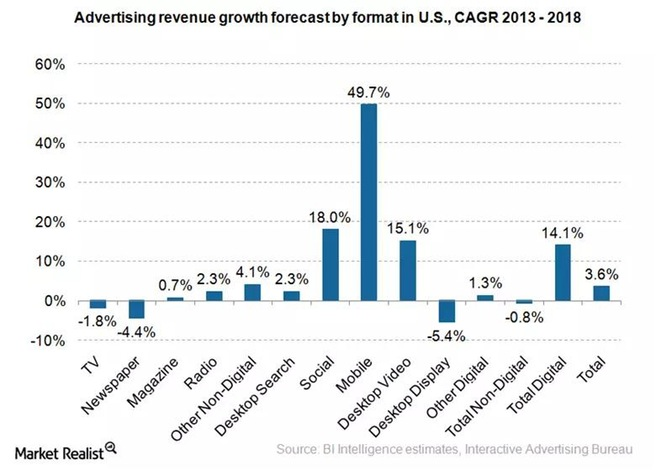
\includegraphics[width=12cm]{img/advRevGrowthFormat}
\caption{Voorspelling groei omzet onderverdeeld per medium}
\label{fig: Advertising revenue growth forecast by format (Business Insider, 2014)}
\end{figure} 

\begin{itemize}
	\item 	Tegen 2019 zal publiciteit op het internet uitgegroeid zijn tot het belangrijkste reclamemedium met een vooropgestelde jaarlijkse groei van 12\%. Verwachte wereldomzet in 2019: 240 miljard dollar. Dit ten nadele van de meer conventionele advertentiemethodieken (krant, tijdschrift, radio, televisie).
	
	\item	Deze groei zal vooral worden gerealiseerd op mobiele toestellen.
	\item	Internetadvertentie technologie zal nog meer toestelbewust worden met als objectief om in alle omstandigheden dicht bij de potentiële klant te zijn (pc, tablet, smartphone, maar ook draagbare interfaces zoals uurwerken).
	\item	Betalende “Search” adverteerders zullen ongeveer 36\% van de totale omzet voor hun rekening nemen (85 miljard dollar).
	\item	Videoadvertentie wordt gezien als mogelijks de belangrijkste toekomstige groeifactor voor de televisiezenders die op computers hun content aanbieden, vooral door de explosieve groei van de internet televisiediensten.
\end{itemize}
Bouwend op deze vooruitzichten zullen er manieren moeten gezocht worden om de inhoud van reclameboodschappen interessant te maken voor de potentiële klant, afgestemd op het gebruikte toestel, en zorgdragend dat dit niet lijdt tot irritaties. 

\chapter{De ad blockers}
\label{ch:De Ad blockers}
De term ad blocker is de overkoepelende term voor alle soorten software die advertenties wegfilteren of verwijderen op een webpagina. Naast het blokkeren van reclame hebben de meest gebruikte ad blockers zoals Adblock Plus en AdBlock nog andere functionaliteiten. Voorbeelden hiervan zijn het uitschakelen van tracking, en het blokkeren van Malware domeinen. Het blokkeren van advertenties zorgt er niet alleen voor dat de gebruiker een aangenamere leeservaring heeft. Een ad blocker zorgt er ook voor dat webpagina’s sneller geladen worden en dat er minder bandbreedte wordt verbruikt. Doordat de reclame wordt geblokkeerd zullen reclamebedrijven ook minder informatie over ad blocker gebruikers ter beschikking krijgen. Met als gevolg dat de privacy beter wordt beschermd. Door het uitschakelen van trackers gaan ad blockers nog een stap verder in het beschermen van de privacy van hun gebruikers.
\section{Aanbieders}
\label{sec:Aanbieders}
\subsection{Adblock Plus}
\label{sec:Adblock Plus}
Adblock Plus\footnote{\url{https://adblockplus.org/}} is een gratis extensie voor Internet Explorer, Mozilla Firefox, Google Chrome, Opera en Safari. Eyeo GmbH is het bedrijf achter Adblock Plus. Over alle browsers heen is dit de meest gebruikte ad blocker met in totaal meer dan 50 miljoen gebruikers\footnote{\url{https://chrome.google.com/webstore/search/ad\%20block?utm_source=chrome-ntp-icon&_category=extensions}} \footnote{\url{https://addons.mozilla.org/nl/firefox/extensions/?sort=users}}. Ondertussen heeft Eyeo ook haar eigen browser voor smartphones ontwikkeld waarmee nu ook advertenties op iPhones of android toestellen geblokkeerd kunnen worden. Anders dan andere ad blockers haalt Adblock Plus zijn inkomsten niet uit donaties. Met hun "`Acceptable ads program"' laten ze bedrijven betalen om hun advertenties op een witte lijst te plaatsen.
\subsection{AdBlock}
\label{sec:AdBlock}
Adblock\footnote{\url{https://getadblock.com/}} is een gratis en opensource extensie voor Google Chrome en Safari. Het team achter AdBlock haalt zijn inkomsten volledig uit donaties. Met in totaal 40 miljoen gebruikers is dit de op één na grootste ad blocker.

\subsection{µBlock Origin}
\label{sec:uBlock Origin}
µBlock Origin\footnote{\url{https://github.com/gorhill/uBlock/}} is een gratis en opensource extensie voor Google Chrome en Mozilla Firefox. µBlock werkt zonder donaties en wordt door een groep vrijwilligers ontwikkeld en onderhouden. Benchmarks door µBlock zelf en \citep{PerformanceAB} tonen aan dat µBlock sneller werkt met een lagere belasting van de CPU. µBlock kan er ook voor zorgen dat scripts enkel uitgevoerd kunnen worden door vertrouwde sites. Tevens is het ook mogelijk om cross-site requests te blokkeren.

\subsection{Ghostery}
\label{sec:Ghostery}
Ghostery is een gratis extensie maar niet opensource. De extensie is beschikbaar voor  Mozilla Firefox, Google Chrome, Microsoft Internet Explorer, Opera, en Safari. Ghostery Inc. is het bedrijf achter de extensie en biedt de extensie gratis aan maar verkoopt de gegevens over de trackers en advertenties die het blokkeert, door aan derden. Ghostery focust zich voornamelijk op het beschermen van de privacy van zijn gebruikers door het blokkeren van trackers, maar verwijdert ook reclame.
\subsection{Brave}
\label{sec:Brave}
Brave is een browser die een ingebouwde ad blocker heeft, en is dus geen extensie die werkt op andere browsers. De browser blokkeert niet alleen reclame en trackers maar vervangt de reclame ook door eigen advertenties. De browser is ontwikkeld door de medeoprichter van het Mozilla Project, het team achter de gelijknamige browser. Brave belooft een stuk van de inkomsten aan advertenties te delen met zowel de gebruikers als de oorspronkelijke adverteerders die hun reclame verwijderd zagen.

\section{Werking van ad blockers}
\label{ch:Werking van ad blockers}
Ad blockers zoals AdBlock en Adblock Plus hebben op zichzelf geen functionaliteit, ze moeten verteld worden wat geblokkeerd moet worden. Dit wordt mogelijk gemaakt door externe filters toe te voegen. Filters zijn in wezen een uitgebreide set van regels die een ad blocker vertellen welke elementen geblokkeerd moeten worden. De meest gebruikte filter is die van EasyList\footnote{\url{https://easylist.adblockplus.org/nl/}}. Alle eerder vernoemde ad blockers gebruiken als basis een filter van EasyList. Deze filters zijn deels regio gebonden, een Nederlandstalige filter zal een grotere focus hebben op Nederlandse en Vlaamse domeinen. Filters zijn regels tekst die bepalen welke adressen niet mogen worden geladen, of welke HTML DOM elementen niet mogen worden getoond.

\subsection{Request blocking}
\label{sec:Request blocking}
De meeste inhoud wordt geblokkeerd door verzoek blocking waarbij ad blockers met behulp van de filters bepalen welke HTTP of HTTPS verzoeken onderschept moeten worden. De filters zijn opgebouwd uit eenvoudige regels. De meest eenvoudige filter die kan gedefinieerd worden is bijvoorbeeld:
\lstset{language=Html,tabsize=2}  
\begin{lstlisting}
http://voorbeeld.com/ads/banner123.jpg
\end{lstlisting}
Je kan deze regel al beter maken door alle banners te blokkeren:
\lstset{language=Html,tabsize=2}  
\begin{lstlisting}
 voorbeeld.com/ads/banner*.jpg 
\end{lstlisting}
 of nog beter:
\lstset{language=Html,tabsize=2}  
\begin{lstlisting}
 http://voorbeeld.com/ads/*.
\end{lstlisting}
Standaard zullen ad blockers voor en na elke regel een wildcard \texttt{'*'} zetten. De filters \texttt{'advertentie'}, \texttt{'ad'} en \texttt{'*ad*'} zijn dan alle drie gelijk. Het is belangrijk hier rekening mee te houden. Wanneer men bijvoorbeeld alle flash bestanden wil blokkeren kan men de filter \texttt{'swf'} toepassen. Maar deze filter zal er ook voor zorgen dat \texttt{'http://voorbeeld.com/swf/index.html'} zal geblokkeerd worden. De oplossing voor dit probleem is het pipe sympool: '|'. Zo zal \texttt{'swf|'} enkel adressen blokkeren die eindigen op 'swf'.
Naast de basisregels zijn er nog meer geavanceerde regels\footnote{\url{https://adblockplus.org/en/filters}}, of kan er gewerkt worden met reguliere expressies. Het gebruik van reguliere expressies wordt sterk afgeraden omdat die de performantie naar omlaag halen.
\\
Wanneer filters die in de meeste gevallen goed werken, toch adressen blokkeren die niet zouden mogen geblokkeerd worden, dan kunnen uitzonderingen gebruikt worden. Als de filter \texttt{'adv'} gebruikt wordt en \texttt{'http://voorbeeld.com/advice.html'} mag niet geblokkeerd worden, dan kan men als uitzondering \texttt{'@@advice'} gebruiken. Uitzonderingsregels verschillen voor de rest niet van de filterregels, en kunnen dus op dezelfde manier samengesteld worden.

\subsection{ Element hidding}
\label{sec:Element hidding}
Soms komt reclame als tekst mee, samen met de opgevraagde webpagina. In dit geval kan de reclame niet geblokkeerd worden door het verzoek te blokkeren. Ad blockers maken dan gebruik van element hidding. Het verstoppen van elementen kan gebruikt worden wanneer de broncode van de webpagina er bijvoorbeeld als volgt uit ziet:
\lstset{language=Html,tabsize=2}  
\begin{lstlisting}
	<div class="textad">
		Goedkoop bier, enkel hier en nu!
	</div>
	<div id="sponsorad">
		Goedkope pizza, klik hier!
	</div>
	<textad>
		Voor goedkoop goud, klik hier!
	</textad>
\end{lstlisting}

Wanneer een webpagina geladen wordt, laadt de reclame automatisch mee. In plaats van de reclame te blokkeren kan men hier enkel de reclame verbergen, zodat die niet zichtbaar is voor de gebruiker. Element hidding regels zijn gelijkaarding opgebouwd als request blocking regels, en beginnen steeds met \texttt{\#\#}. Daarnaast worden de regels opgebouwd met behulp van css selectors. In bovenstaand geval kan men bijvoorbeeld als regel \texttt{\#\#div.textad} gebruiken om het eerste reclameblok te verwijderen. Voor het tweede reclameblok en specifiek voor één domein wordt volgende regel gebruikt: \texttt{example.com\#\#div\#sponsorad}.

Sommige ad blockers zoals Adblock Plus en µBlock Origin beschikken over een handige tool die toelaat om manueel elementen te verbergen met behulp van een selector. Via een eenvoudige muisklik kan men de elementen kiezen die men liever verborgen wil zien. De ad blocker zal dan automatisch een regel genereren die bij het geselecteerde element hoort.

\section{Business model}
\label{sec:Business model}
Het business model van de instanties achter ad blockers verschilt sterk van organisatie tot organisatie. Er zijn ad blockers zoals µBlock Origin die volledig open source zijn en zelfs donaties weigeren. Daarnaast zijn er bedrijven zoals AdBlock die wel op zoek gaan naar donaties. Anderen zoals Ghostery verzamelen, als de gebruiker hier in toestemt, informatie over de trackers en reclames op de websites die bezocht worden. Die verzamelde data verkopen ze dan door aan derden. Het is belangrijk om te benadrukken dat ze geen gebruikersinformatie verzamelen, maar wel informatie over de bezochte website en bijhorende trackers.
\subsection{ Accepteable ad's program}
\label{sec:Accepteable ad's program}
Naast bovenstaande methodes is er nog een andere manier om geld te verdienen aan ad blocking, namelijk geld vragen aan adverteerders om hun advertenties niet te blokkeren. Dit is het business model van Adblock Plus. Deze manier van werken is omstreden omdat hun Accepteable ad's program procedure verdacht veel lijkt op afpersing. Eén van de grote hekelpunten was oorspronkelijk dat het systeem niet transparant genoeg werkte. Pas in december 2016 is Adblock Plus voor het eerst open geweest over hoe ze hun inkomsten vergaren. Sindsdien is op hun website een apart topic te vinden waarin uitgelegd wordt hoe ze gefinancierd worden. 
\\
\\
Een deel van de inkomsten verkijgen ze nog steeds via donaties van gebruikers.
Maar de grootste bron van inkomsten gebeurt via het acceptabele advertentie programma waarin ze webpagina's aan een whitelist toevoegen. De advertenties die zich bevinden op de websites die op die whitelist staan, worden niet geblokkeerd. 
Adblock Plus maakt voor whitelisting een onderscheid tussen grote en kleine advertentie-eenheden. Een eenheid wordt als groot beschouwd als er een winst is van meer dan 10 miljoen extra advertentievertoningen per maand, door deelname aan het Acceptable Ads initiatief. Slechts 10\% van de whitelisting certificaten behoren tot de groep ‘grote ondernemingen’. Deze grote eenheden betalen een licentievergoeding voor het plaatsen van advertenties op de lijst. Deze vergoeding bedraagt normaal gesproken 30\% van de extra inkomsten die behaald worden door de whitelisting. 90\% van de certificaten worden echter gratis toegekend aan kleinere advertentie-eenheden. Het betalen van een licentievergoeding staat volledig los van de criteria om toegelaten te worden op de whitelist. Zolang de Acceptable Ads criteria niet voldaan zijn, is er geen sprake van whitelisting. Er is dus geen enkele mogelijkheid om voor een advertentie die niet aan de Acceptable Ads criteria (zie hoofdstuk \ref{sec Het acceptabele advertentie manifesto}) voldoet, een plaatsje op de lijst te kopen.

Om de transparantie naar de buitenwereld te vergroten heeft Adblock Plus besloten om alle whitelisted advertenties en deelnemende eenheden publiek te maken op het forum van Adblock Plus \footnote{\url{https://adblockplus.org/forum/viewforum.php?f=12}}.
De inkomsten van de licentievergoedingen worden onder andere gebruikt voor het onderhouden van het acceptabele advertentie programma. Er werken vrijwilligers aan mee via de Adblock Plus forum community, maar het grootste deel van het beheer van de lijst (contacten met adverteerders, voortdurende controle, technische ondersteuning, …) wordt gedaan  door Eyeo GmbH, het bedrijf achter Adblock Plus.


\chapter{Evolutie gebruik Ad blockers}
\label{ch:Evolutie gebruik Ad blockers}

\section{Groei}
\label{sec:Groei}
Eind 2015 werd wereldwijd de kaap van 200 miljoen maandelijks actieve ad block gebruikers overschreden \citep{PageFair2015}. Over het volledige jaar 2015 waren er bijna 3.2 miljard\footnote{\url{ http://www.internetlivestats.com/internet-users/\#trend}} actieve internetgebruikers. Dit betekent dat meer dan 6.25\% van de internetgemeenschap een ad blocker gebruikt. Verwacht wordt dat dit percentage de komende jaren enkel maar zal stijgen. Wanneer de trend van de voorbije jaren zich voortzet, zal het aantal gebruikers van een ad blocker jaarlijks met meer dan 40\% blijven stijgen \ref{fig: adblock-growth}.
\begin{figure}[h!]
\centering
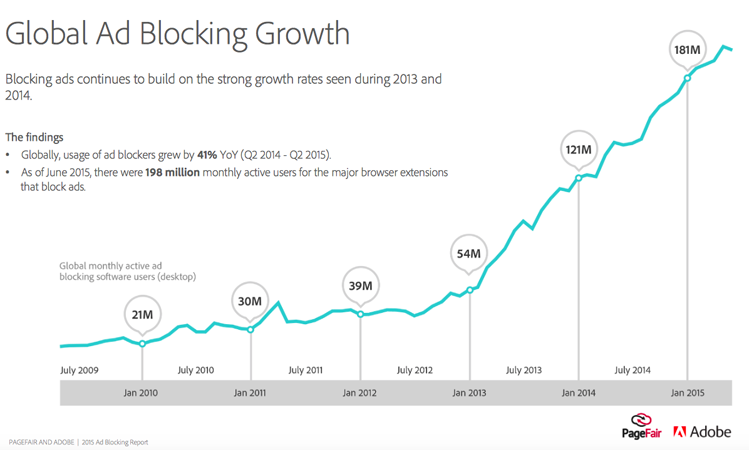
\includegraphics[width=12cm]{img/adblock-growth}
\caption{Evolutie maandelijks actieve ad block gebruikers (Pagefair, 2015)}
\label{fig: adblock-growth}
\end{figure}



\section{Spreiding}
\label{sec:Spreiding}
In 2014 en opnieuw in 2015 verzamelde PageFair samen met Adobe informatie omtrent het gebruik van ad blockers \citep{PageFair2015,PageFair2014}.

\subsection{Demografische spreiding}
\label{sec Demografische spreiding}
Ad block gebruikers zijn voor het grootste deel mannen. Het is 48\% waarschijnlijker dat een man een ad blocker gebruikt bij het browsen dan een vrouw, figuur: \ref{fig: Demographic_age_sex}. Wat betreft leeftijd zijn voornamelijk tieners of jonge twintigers de grootste gebruikers van ad blockers. Van de ondervraagde personen tussen 18 en 29 jaar gaf maar liefst 41\% toe een ad blocker te gebruiken. Daar komt nog eens bij dat het ook deze groep is die het meest gebruik maakt van het internet, figuur:\ref{fig: adbvsnadbHoursofIntertnet}. Het aandeel in het aantal actieve ad block gebruikers daalt met de leeftijd.

\begin{figure}[p]
\centering
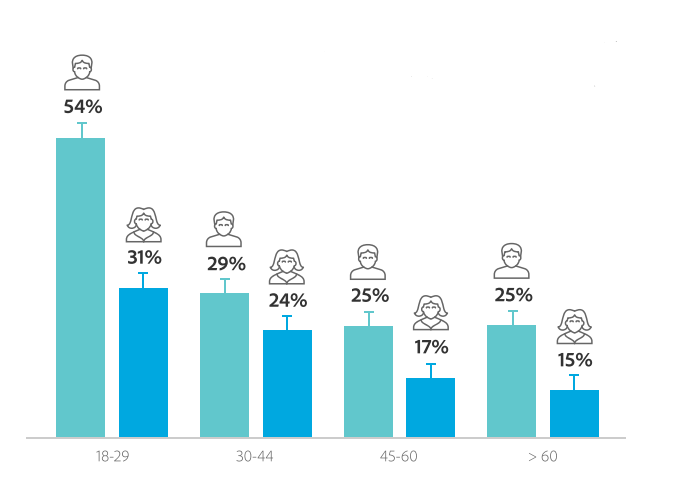
\includegraphics[width=12cm]{img/demographicsMV}
\caption{Ad block gebruikers volgens leeftijd en geslacht (Pagefair, 2014) }
\label{fig: Demographic_age_sex}
\end{figure}

\begin{figure}[p]
\centering
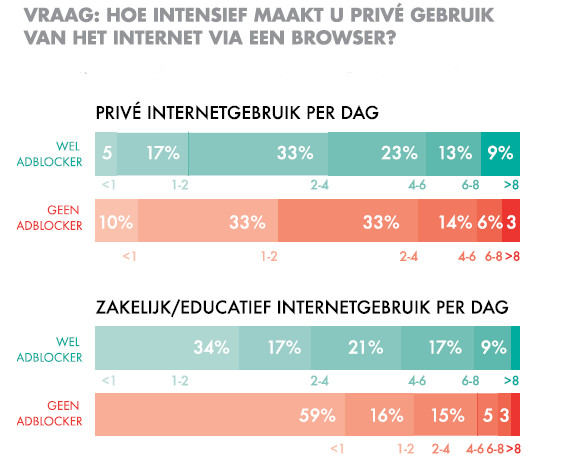
\includegraphics[width=12cm]{img/adbvsnadbHoursofIntertnet}
\caption{Gemiddeld aantal uren internet per dag, (IAB NL, 2015) }
\label{fig: adbvsnadbHoursofIntertnet}
\end{figure}



\subsection{Geografische spreiding}
\label{sec Geografische spreiding}
Ad block gebruikers bevinden zich vooral in Europa en Noord-Amerika. Ad blocker gebruik is nog niet echt doorgedrongen in Azië\footnote{\url{www.techinasia.com/adblock-plus-in-asia}}.
Griekenland en Polen zijn in Europa veruit de grootste gebruikers van ad blockers (respectievelijk 37\% en 35\%). België bengelt achteraan in de lijst met 12\%, en laat enkel Tsjechië, Frankrijk en Sovakije (8.9\%) achter zich, figuur: \ref{fig: ratespercountry}.
\begin{figure}[h!]
\centering


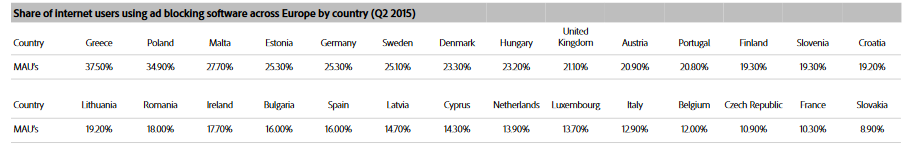
\includegraphics[width=16cm]{img/ratespercountry}
\caption{Ad block gebruik in Europa per land (Pagefair, 2015)}
\label{fig: ratespercountry}
\end{figure}

\subsection{Spreiding over de verschillende browsers}
\label{sec spreiding over de verschillende browsers}
De desktop internetbrowsers Chrome en Firefox hebben het grootste percentage actieve ad block gebruikers, figuur: \ref{fig: Ad-blocking-by-browse}. Meer dan 35\% van de gebruikers van Firefox gebruiken een ad blocker en daarmee ligt deze browser op kop. Het aantal maandelijks actieve gebruikers ligt bij Chrome wel een stuk hoger op 126 miljoen ten opzichte van de 48 miljoen van Firefox. Het gebruik van ad blockers zag bij Chrome ook een grotere toename in vergelijking met andere browsers, het gebruik steeg van 2014(Q2) naar 2015(Q2) met 51\%. Dit heeft enerzijds te maken met het gemak waarop in deze browser ad blockers kunnen gebruikt worden, maar ook met het feit dat meer en meer internetgebruikers overschakelen naar Chrome, figuur: \ref{fig: UsersPerBrowser}.
\begin{figure}[h!]
\centering
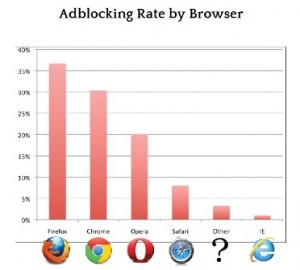
\includegraphics[width=12cm]{img/Ad-blocking-by-browse}
\caption{Percentage Ad blocker gebruikers per browser (Forbes, 2013)}
\label{fig: Ad-blocking-by-browse}
\end{figure}

\begin{figure}[h!]
\centering
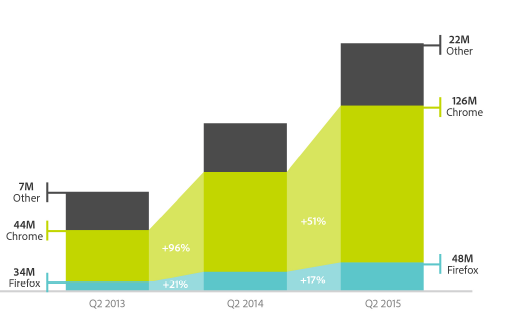
\includegraphics[width=12cm]{img/UsersPerBrowser}
\caption{Groei maandelijks actieve gebruikers (Pagefair, 2015)}
\label{fig: UsersPerBrowser}
\end{figure}


\newpage
\subsection{Spreiding over de verschillende content}
\label{sec Spreiding over de verschillende content}
Bij websites met een technisch gekwalificeerder publiek kan het gebruik van een ad blocker door de bezoekers meer de regel zijn dan de uitzondering. Gaming en social network sites hebben het hoogste ad blocking percentage: respectievelijk 26.5\% en 19.3\%, figuur:\ref{fig: percontent}. Het hoge percentage voor gaming sites ligt in lijn met het hoge percentage dat de jonge groep mannen haalt in het demografisch onderzoek. Officiële websites van overheidsinstellingen hebben het laagste percentage : 2.5\%.

\begin{figure}[h!]
\centering
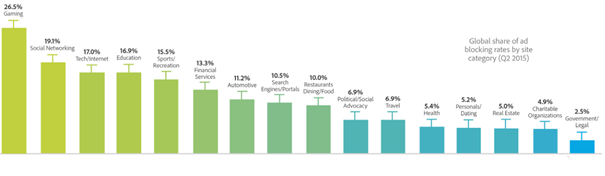
\includegraphics[width=15cm]{img/percontent}
\caption{Het aandeel van ad blockers per content (Pagefair, 2015)}
\label{fig: percontent}
\end{figure}

\subsection{Mobiel gebruik van ad blockers}
\label{sec Mobiel gebruik van ad blockers}
Er is een verschuiving zichtbaar van het percentage van internet gebruik op desktop naar dat op smartphone of tablet, figuur: \ref{fig: MobileVsDeskotpInternet}. In 2015(Q2) werd 38\% van alle webbrowsing op smartphone of tablet uitgevoerd. Verwacht wordt dat eind 2016 de kaap van 50\% bereikt wordt. Voor sommige websites zoals YouTube komen nu al meer dan de helft van de bezoeken via mobiele toestellen \footnote{\url{youtube.com/yt/press/statistics.html}}. Momenteel wordt slechts 2\% van de advertenties op de mobiele toestellen geblokkeerd, \cite{PageFair2015}. Enkel in Azië ligt dat percentage een stuk hoger met uitschieters als China en India met respectievelijke 7.9\% en 9.0\%. 
Op mobiele toestellen zijn er voor de gebruiker twee manieren om digitale inhoud te bekijken: via een mobiele browser of via apps. Anders dan voor desktop browsers kan er voor mobiele browsers geen ad blocker plug-in geïnstalleerd worden. Er moet een aparte browser worden gedownload die de ad block functionaliteit heeft ingebouwd. Gebruikers nemen niet graag afscheid van hun favoriete browser. Daarnaast zijn er ook ad blockers die advertenties van de apps blokkeren, maar deze ad blockers werken nog niet optimaal. Ad blocking op mobiele toestellen is dus zeker mogelijk maar staat nog in zijn kinderschoenen.
Doordat advertenties soms tot meer dan de helft\footnote{\url{http://www.nytimes.com/interactive/2015/10/01/business/cost-of-mobile-ads.html}} van de bandbreedte verbruiken op mobiele toestellen zijn mobiele providers bezig met de ontwikkeling van een ad blocker die ingebouwd is in hun netwerk. Het Israëlische bedrijf Shine biedt een technologie aan die dit mogelijk maakt. Voorlopig is er nog maar één Europese provider die het systeem gebruikt.


\begin{figure}[h!]
\centering
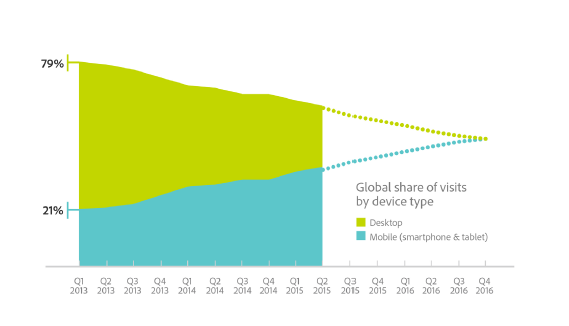
\includegraphics[width=12cm]{img/MobileVsDeskotpInternet}
\caption{Evolutie bezoeken per type toestel (Pagefair, 2015)}
\label{fig: MobileVsDeskotpInternet}
\end{figure}

\subsection{Conclusie}
\label{sec Conclusie}
De gemiddelde ad block gebruiker is een man tussen 18 en 29 jaar en woont in Noord-Amerika of West-Europa. Dit is tevens de groep die het meest gebruik maakt van het internet. Dit zou dan ook een verklaring kunnen zijn waarom slechts 6.25\% van de internetgemeenschap een ad blocker gebruikt, maar het aantal geregistreerde ad block gebruikers bij veel websites een stuk hoger ligt. Momenteel is ad blocking voor mobiele toestellen nog geen wijdverspreid fenomeen. Maar door de verbetering van de huidige technologie en door nieuwe technologieën wordt verwacht dat het aantal ad blockers op mobiele toestellen sterk zal stijgen.

\section{Redenen voor gebruik ad blocker}
\label{sec:Redenen voor gebruik ad blocker}
Naast het blokkeren van reclame zijn er nog een aantal andere reden waarom mensen ad blockers gebruiken. Ad blockers zorgen voor een extra laag beveiliging, ze zorgen ervoor dat webpagina's sneller worden geladen, beschermen de privacy en er wordt ook minder bandbreedte verbruikt, \cite{IAB2014}.

%\begin{figure}[h!]
%\centering
%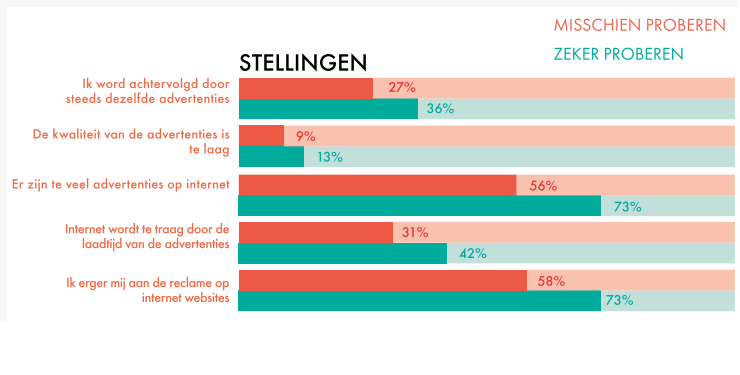
\includegraphics[width=12cm]{img/redenadblockgebruik}
%\caption{Grootste ergernis van reclame op het internet in Nederland}
%\label{fig: redenadblockgebruik}
%\end{figure}

\subsection{Reclame}
\label{sec Reclame}
Net zoals de meeste mensen geneigd zijn om bij televisiereclame, met de afstandsbediening naar een andere zender over te schakelen, wil men bij het gebruik van internet ook de mogelijkheid hebben om advertenties te ontlopen. Vooral advertenties die de ervaring van de bezoeker verstoren zijn een reden om een ad blocker te installeren, \cite{IABNL2015}. De grootste ergernis vormen advertenties die niet weggeklikt kunnen worden (59\%), deze die de website grotendeels bedekken (54\%) en de advertenties met geluid (41\%), figuur: \ref{fig: Redenadblockreclame}.
\begin{figure}[h!]
\centering
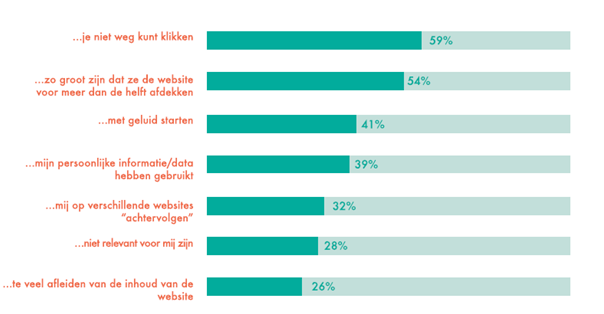
\includegraphics[width=12cm]{img/Redenadblockreclame}
\caption{Ergernis van gebruikers per soort reclame, (IAB NL, 2015)}
\label{fig: Redenadblockreclame}
\end{figure}

\subsection{Clickbait}
\label{sec click bait}
Clickbait (letterlijke vertaling: ‘klikaas’) is een internetjournalistiek die inspeelt op de nieuwsgierigheid van de lezer. Ze maakt gebruik van vage, sensationele koppen in een poging om de lezer tot een klik te verleiden. De lezer wordt dan naar een site geleid vol reclame, en meestal weet het artikel de sensatie van de kop niet eens waar te maken. De site staat ook vol van andere artikels met al even spectaculaire koppen, in de hoop dat de bezoeker zich opnieuw laat vangen.
\\
Voorbeelden van clickbait zijn:
\lstset{columns=flexible}
\begin{lstlisting}
	-Mensen kunnen duizend jaar worden
	-10 manieren om nooit meer moe te zijn
\end{lstlisting}


\subsection{Tracking/privacy}
\label{sec tracking/privacy}
Men zou verwachten dat de irritatie die sommige advertenties opwekken de grootste reden is om over te gaan tot ad blocking. Maar uit het onderzoek van Pagefair in samenwerking met Adobe, \cite{PageFair2015}, blijkt dat privacy de belangrijkste reden is voor het installeren van een ad blocker. De gebruikers willen niet dat persoonlijke informatie verzameld, geanalyseerd en gebruikt wordt door de adverteerders. Bij elke browsingsessie zijn er honderden firma's die online activiteit en browsing historiek volgen, en bewaren. Dit is de reden dat als men eens een artikel opgezocht heeft, men blijft achtervolgd worden door advertenties die verband houden met dit artikel. Ad blockers kunnen ingezet worden om deze tracking te vermijden. Daarvoor wordt net als voor het verwijderen van advertenties gebruik gemaakt van filterlijsten. EasyPrivacy Tracking Protection \footnote{\url{https://easylist.adblockplus.org/nl/}} List is een optioneel aanvullend abonnement, waarbij alle vormen van tracking van het internet worden verwijderd. Dit gebeurt inclusief web bugs, tracking scripts en andere informatieverzamelende elementen. Daardoor worden je persoonlijke gegevens beter beschermd.

\subsection{Beveiliging}
\label{sec Beveiliging}
Ad blockers zijn in staat je computer te beschermen tegen malvertising. Malvertising zijn advertenties die opzettelijk bewerkt zijn met malware om de computers te besmetten van iedereen die de site waarop de advertentie staat bezoekt. Dit kan gebeuren ook al wordt de besmette advertentie niet eens aangeklikt. 
In de advertentie zit een stuk code dat zelfs zonder dat de advertentie geladen wordt, de computerbeveiliging van de gebruikers onderzoekt. In die code wordt beslist welk stuk van malware doorgestuurd wordt naar de computer. Er worden stukken software (adware) geïnstalleerd op de harde schijf. Deze stellen de computer open voor gegevensdiefstal en andere cybercriminaliteit. Als de computer door malware geïnfecteerd is, zijn gegevens voor online bankieren, kredietkaartinformatie, wachtwoorden en andere gevoelige gegevens niet meer veilig. 
Ad blockers kunnen dus gebruikt worden om zichzelf te beschermen tegen malware (Trojan horses, wormen, spy- en adware en andere virussen). Het uitschakelen van bekende malware domeinen wordt gedaan door een nieuw filterabonnement, Malware Protection, toe te voegen. Maar een ad blocker is geen gespecialiseerd antivirusprogramma. Het is niet aan te raden speciaal ontworpen antivirusprogramma's te vervangen door een ad blocker. 

\subsection{Laadsnelheid en bandbreedte}
\label{sec Laadsnelheid en bandbreedte}
De laadsnelheid van een pagina is de tijd die nodig is om een pagina volledig te laden nadat een gebruiker de pagina heeft geopend. De bandbreedte die de webpagina verbruikt, is het aantal MegaByte dat geladen wordt bij het openen van een pagina. Bandbreedte is vooral van belang wanneer de verbinding met het internet over een connectie verloopt waarbij elke verbruikte MegaByte aangerekend wordt, zoals smartphones en andere mobiele apparaten. Ook snelheid is voor mobiele apparaten van belang want hoe langer het duurt voor om een webpagina te laden, hoe sneller de batterij zal leeglopen. Doordat ad blockers de reclame tegenhouden, zal de laadsnelheid stijgen en het data verbruik dalen.
\\

Uit eigen onderzoek, \ref{fig: LoadTimes} kunnen we afleiden dat er kleine tot zeer grote verschillen in webpagina laadtijd worden vastgesteld wanneer een ad blocker (Adblock Plus) wordt gebruikt. Gemiddeld wordt een 15\% minder paginalaadtijd genoteerd wanneer een ad blocker wordt gebruikt. Er kon ook worden vastgesteld dat het verschil in laadtijd kleiner wordt naarmate er minder advertentie worden ingelast.

\begin{figure}[h!]
\centering
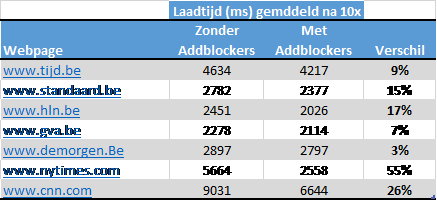
\includegraphics[width=12cm]{img/Eigenonderzoek}
\caption{Laadtijden met en zonder ad blocker}
\label{fig: LoadTimes}
\end{figure}

Uit een onderzoek (\cite{Fraser2015}) blijkt dat de installatie van Adblock Plus het gebruik van bandbreedte met 25\% naar omlaag brengt. Wanneer de ad content ook videobeelden bevat, dan loopt de winst zelfs op tot 40\%. 

The New York Times deed ook een onderzoek naar de impact van ad blockers op mobiele toestellen, \cite{nytimes2015}.
In dit onderzoek werden 12 belangrijke nieuwswebsites betrokken. De gegevens van het dataverkeer van zowel de advertenties als de reële krantenartikels werden onderzocht. Elke startpagina werd 10 maal geladen, verspreid over 2 dagen, op een Iphone 6, met 4G mobiel netwerk. Dit gebeurde eens met de ad blocker geactiveerd, en eens gedeactiveerd. Een tweede test werd gedaan om de invloed op de levensduur van de batterij te testen. Een speciale app werd ontwikkeld om door tientallen populaire websites te gaan, in een eindeloze loop. Er werd dan getimed hoe lang het duurde voor de batterij volledig leeggelopen was.

De laadtijd voor The New York Times zonder ad blocker bedraagt 7 seconden voor 3.7 MB data. Door het weglaten van de advertenties door een ad blocker , verlaagt dit tot 4 seconden voor 2.1 MB data. Het opvallendste verschil was te merken bij Boston.com. Met advertenties was er 19.4 MB data. Als de advertenties verwijderd waren door ad blocker Crystal was er 4 MB data, met 1Blocker 4.5 MB. Door het weglaten van de advertenties door een ad blocker , verlaagt de laadtijd van 39 seconden naar 8 seconden.
Ongeveer de helft van het dataverkeer komt van de advertenties, en wordt uitgefilterd bij gebruik van een ad blocker. Dit dataverkeer is ook duur. Er wordt geschat dat op een gemiddeld mobiel data-abonnement, elke megabyte gedownload via een mobiele netwerk, ongeveer 1 dollarcent kost . Een dagelijks bezoek aan bijvoorbeeld de startpagina van Boston.com gedurende een maand, zou ongeveer 9.5 dollar kosten, enkel voor het dataverkeer van de advertenties. 
Uit het onderzoek valt ook op te maken dat ad blocking inschakelen op je smartphone de levensduur van je batterij met ongeveer 20\% verhoogt. Maar deze winst geldt alleen voor de tijd dat je web browsing doet op je smartphone.
\\
Voor een aantal websites die advertenties met veel data bevatten, daalt het dataverkeer aanzienlijk als ad blockers ingeschakeld zijn. De laadtijden versnellen enorm, en de levensduur van de smartphonebatterij verhoogt ook, maar meer bescheiden.

\subsection{Conclusie}
\label{sec Conclusie}
De grootste motieven voor mensen die overwegen een ad blocker te installeren zijn: het beschermen van hun privacy tegen reclamenetwerken, irritatie over (te veel) advertenties, en een te trage performantie. Dit zijn eveneens de werkpunten waar de reclamenetwerken in de toekomst best rekening mee houden. 

\chapter{Impact van ad blockers}
\label{ch: Impact van ad blockers}

\section{Impact op de websites}
\label{sec:Impact op de webpagina's}
Advertenties zorgen vaak voor een groot stuk van de inkomsten op websites. Sommige websites zijn zelfs volledig afhankelijk van advertenties voor hun inkomsten. De adverteerders betalen voor de infrastructuur en betalen de mensen die instaan voor het onderhoud en de inhoud van een website. Wereldwijd werd er in 2015 149.2 miljard dollar gespendeerd aan internetreclame. Het totale verlies aan reclame-inkomsten door ad blockers bedroeg in 2015 21.88 miljard dollar, \cite{PageFair2015}. Websites lopen globaal gezien dus bijna 13\% van hun inkomsten mis door ad blockers. 
\\
Uit interviews met verschillende content creators op YouTube en nieuwswebsites blijkt dat het verlies aan inkomsten ongelijkmatig verdeeld is. Bij een Youtuber genaamd Driftor, die voornamelijk video's maakt die gerelateerd zijn aan videogames, loopt het verlies aan inkomsten soms op tot 45\%. Dit ligt in lijn met de onderzoeksresultaten uit hoofdstuk \ref{sec Spreiding over de verschillende content}, waaruit blijkt dat websites met een grote focus op videogames het grootste percentage ad block gebruikers hebben. 
Ook een andere Youtuber genaamd Barnacules Nerdgasm, die video's maakt met een zeer technische inhoud en met onderwerpen zoals Bitcoins en 3D printing, ziet meer dan 16\% van zijn inkomsten verloren gaan. Uit het interview met Barnacules blijkt dat 35\% van zijn doelpubliek op pc een ad blocker gebruikt. Dit aantal  is echter al meer dan een jaar constant doordat een groot stuk van zijn publiek overschakelt naar mobiele toestellen om zijn video's te bekijken. Doordat het gebruik van ad blockers op smartphones nog niet ingeburgerd is, kan hij het verlies aan inkomsten door het stijgend aantal ad blockers op desktop compenseren.

Uit een interview met Peter Soetens, directeur digitale nieuwsmedia van Mediahuis nv, blijkt dat ook bij hen het verlies aan inkomsten meevalt door het steeds groter aandeel van mobiele bezoekers. Mediahuis is een Belgisch mediabedrijf dat naast kranten zoals De Standaard, Het Nieuwsblad en de Metro ook websites zoals Jobat beheert. Dagelijks heeft Mediahuis 1.3 miljoen digitale bezoekers waarbij op desktop 18\% van de bezoekers een ad blocker gebruikt, en op mobiel minder dan 1\% een ad blocker gebruikt. Peter Soetens wist te zeggen dat het gebruik van ad blockers zeker een zorgenkind is, maar zolang het gebruik bij mobiele toestellen laag blijft, vormen ad blockers geen echte bedreiging voor Mediahuis.

\section{Impact op de adverteerders}
\label{sec:Impact op de adverteerders}
De meeste adverteerders betalen per impressie of per doorklik. Ze betalen dus geen op voorhand vastgelegde som. Dit betekent dat er niet moet betaald worden voor advertenties die niet worden gezien door gebruikers omdat deze een ad blocker geactiveerd hebben. Adverteerders bereiken door ad blocking een kleiner publiek, maar betalen daardoor ook minder. 
Een groter nadeel is het feit dat ze door het kleinere bereik, ook van minder mensen gegevens kunnen verzamelen, en daardoor minder efficiënt reclame kunnen maken.
Het wordt een nieuwe uitdaging voor adverteerders om advertenties te maken die de gebruiker minder irriteren, zodat minder snel naar een ad blocker gegrepen wordt.
Ook de beheerders van websites zijn kritischer geworden over de kwaliteit van de advertenties op hun webpagina’s. Ook zij hebben er baat bij dat zo weinig mogelijk gebruikers kiezen voor een ad blocker.

\section{Impact op de internetgebruiker}
\label{sec:Impact op de internet gebruiker}
Bij het initieel invoeren van reclame op internet, hadden sommige websitebeheerders het moeilijk om voor elke bezoeker de advertentieruimte volledig in te vullen. Zelfs met de komst van reclamenetwerken en exchange netwerken, werd de reclameruimte per gebruiker maar zelden volledig benut. Door de komst van ad blocking wordt het aantal bezoekers dat de reclame te zien krijgt kleiner.  Tegelijk wordt het voor de websitebeheerders eenvoudiger om de advertentieruimte voor elke gebruiker meer en meer in te vullen. Meer advertenties heeft als gevolg dat gebruikers die nog geen ad blocker hebben nu misschien toch geneigd zijn om er zich één aan te schaffen. Men kan dus spreken van een soort vicieuze cirkel waar men in terechtkomt.
Peter Soetens bevestigde ook dat sinds het gebruik van ad blockers, de mensen die geen ad blocker gebruiken, een groter aanbod aan reclame voorgeschoteld krijgen.

\section{Impact op de advertenties}
\label{sec:Impact op de advertenties}
Websites zijn steeds meer vragende partij naar betere reclame, zodat gebruikers minder snel naar een ad blocker grijpen. Het is ook bij de reclamenetwerken doorgedrongen dat de stijl van adverteren moet veranderen om geaccepteerd te blijven worden.
\subsection{Het L.E.A.N. advertentie programma}
\label{sec Het L.E.A.N. advertentie programma}
 Het IAB introduceerde in 2015 het L.E.A.N. advertentieprogramma als antwoord op het stijgend aantal ad block gebruikers. L.E.A.N. staat voor: light, encrypted, ad choice support en non-invasive ads (licht, versleuteld, ondersteuning voor keuze en niet invasieve advertenties). Ze willen daarmee de redenen voor gebruik van ad blockers aanpakken, zie hoofdstuk \ref{sec:Redenen voor gebruik ad blocker}. In een artikel van het IAB (Lean2015) staat dat het mede door de schuld van adverteerders is dat ad blockers zo veel gebruikt worden. Adverteerders waren in de zoektocht naar zo efficiënt mogelijk adverteren de gebruikerservaring uit het oog verloren. Met het L.E.A.N. programma wil IAB zo veel mogelijk adverteerders overtuigen om advertenties van een hogere standaard te maken. Het IAB kan netwerken natuurlijk niet verplichten om betere reclame te maken. Maar reclamereus Google heeft al gezegd hun advertenties aan te passen voor een betere gebruikerservaring\footnote{\url{digiday.com/publishers/google-said-exploring-acceptable-ads-policy/}}. Andere reclamenetwerken beginnen het voorbeeld van Google en IAB te volgen.

\subsection{Het acceptabele advertentie manifesto}
\label{sec Het acceptabele advertentie manifesto}
Adblock Plus was de eerste ad blocker die toeliet om advertenties die aan bepaalde voorwaarden voldoen op een witte lijst te zetten. De voorwaarden voor op de witte lijst te komen zijn de volgende:

\begin{itemize}
	\item Plaatsing: boven, onder of opzij van de primaire inhoud van een webpagina.
	\item Onderscheid: de advertentie moet herkenbaar zijn als reclame, en mag niet te beschouwen zijn als deel van de primaire inhoud van een webpagina.
	\item Grootte: er zijn verschillende restricties in afmetingen voor de advertenties naargelang de plaats.
	\item Voor tekstadvertenties: overmatig gebruik van kleuren of andere elementen die overdreven de aandacht trekken zijn niet toegelaten
	\item Voor beeldadvertenties: statische beeldadvertenties worden aanvaard als ze onopvallend geïntegreerd zijn in de webpagina
\end{itemize}

De volgende advertenties maken nooit kans om als acceptabele advertentie beschouwd te worden:

\begin{itemize}
	\item Advertenties die andere advertenties inladen. 
	\item Advertenties met overdreven effecten.
	\item Advertenties met animaties.
	\item Advertenties die automatisch geluid of video afspelen.
	\item Advertenties die vóór of tijdens het laden worden getoond.
	\item Pop-ups en pop-unders.
	\item Videoreclame die afspeelt vóór je de inhoud van de webpagina kunt bekijken.
\end{itemize}

\section{Conclusie}
\label{sec Conclusie}
Veel advertentiebedrijven begrijpen de redenen voor gebruik van ad blockers. Deze zijn snelheid, privacy, beveiliging en een webpagina zonder afleidingen. Ze beginnen te beseffen dat voor een internet met reclame, de reclame minder agressief en storend moet worden. Voorlopig ondervinden sommige websites meer last van ad blockers dan anderen. Bij velen valt het verlies aan inkomsten voorlopig mee doordat veel gebruikers overschakelen naar mobiele toestellen zonder ad blockers. Veel makers van content zien momenteel ad blockers op mobiele toestellen als grootste bedreiging voor hun inkomsten.


\chapter{Hoe wapenen bedrijven zich tegen ad blockers}
\label{ch:Hoe wapenen bedrijven zich tegen ad blockers}
In een poging om terug te vechten tegen het steeds groeiend gebruik van ad blockers, gebruiken websites die overleven op inkomsten uit reclame verschillende technieken. Dit varieert van meldingen die inspelen op het geweten van de bezoekers van de webpagina, tot het volledig blokkeren van toegang tot de pagina voor bezoekers die een ad blocker geactiveerd hebben.
\\
Voor de eigenaar of beheerder van een webpagina zijn er verschillende mogelijkheden:

\begin{itemize}
	\item Een gebruiker van een ad blocker detecteren en vervolgens de toegang weigeren.
	\item Gebruik maken van een paywall, waarbij enkel betalende gebruikers toegang tot de content hebben. Een gelimiteerd aantal gratis bezoeken/artikels alvorens te vragen om te abonneren, verlaagt de drempel 
	\item Gebruikers om een vrijblijvende donatie vragen, als vervanging voor de verloren inkomsten door het gebruik van een ad blocker.
	\item Gesponsorde content.
	\item Native adverteren.
\end{itemize}

De beste keuze is afhankelijk van verschillende factoren. Bijvoorbeeld de inhoud van een webpagina en de loyaliteit van haar bezoekers. De grootte van de impact die reclame heeft op de inkomstenstroom van de website is ook belangrijk. Bij een webpagina die zich focust op verkoop van goederen of diensten zou het niet productief zijn om mensen die een ad blocker gebruiken te blokkeren. Het vragen naar donaties zal ook negatief overkomen. Zelfs een melding met de vraag om de ad blocker uit te schakelen zal de gebruiker als onaangenaam ervaren.

\section{Blokkeren van ad block gebruikers}
\label{sec Blokkeren van ad block gebruikers}
Wanneer de verliezen van reclame-inkomsten te groot worden, kan er voor gekozen worden om gebruikers van ad blockers toegang tot de webpagina te ontzeggen. Dit kan zolang de ad blocker actief is, of tot wanneer de webpagina wordt toegevoegd aan de whitelist van de ad blocker. 
\\
Het idee achter deze aanpak kan gevaarlijk zijn: in veel gevallen zien inhoud-aanbieders ad blocker gebruikers als niet belangrijk of niet waardevol. Ze profiteren immers van de website zonder iets in ruil te geven. Maar ze lopen zo het risico veel verkeer en de loyaliteit van de gebruiker te verliezen. Vooral bij nieuwssites waarbij het aanbod zeer uitgebreid is, is dit van belang. Het is de loyaliteit die er voor zorgt dat gebruikers altijd blijven terug komen naar een specifieke webpagina, en het is die loyaliteit die er in de toekomst voor kan zorgen dat gebruikers een abonnement kopen. Op lange termijn zou het dus kunnen zijn dat gebruikers blokkeren een negatief effect heeft.
\\
Wanneer men de mogelijke gevolgen op lange termijn negeert, zorgt het blokkeren van gebruikers van ad blockers effectief voor het gewenste resultaat. Volgens een onderzoek van IAB(Internet Advertising Bureau) in het Verenigd Koninkrijk, zouden 64\% van de ondervraagden hun ad blocker uitschakelen wanneer toegang wordt geweigerd. Hieruit kan ook worden afgeleid dat 30-40\% van ad block gebruikers dit niet doen en dus wegblijven van websites die hen de toegang blokkeren. De kans dat ze dan in de toekomst terugkeren naar de website is klein. Vooral voor websites die naast hun advertenties hun inkomsten halen uit andere producten of diensten kan dit nadelig zijn.
\\
Een ander probleem zijn de beperkte technische mogelijkheden voor het detecteren en blokkeren van ad block gebruikers. Deze technieken maken gebruik van scripts die naar verloop van tijd omzeild worden door sommige ad blockers zoals µBlock. Voor sommige andere ad blockers lukt het niet om deze technieken te omzeilen, maar een extra plugin, Anti-Adblock killer, downloaden en installeren volstaat om de blokkering te omzeilen.
\\
De enige technologie die er tot nu toe altijd in slaagde om elke ad blocker te detecteren is BlockAdblock \footnote{\url{http://blockadblock.com/}}. De wetgeving inzake privacy speelt hier ook een grote rol, zie hoofdstuk \ref{ch: Wetgevingen en rechtzaken rond ad blockers}.

\begin{figure}[h!]
\centering
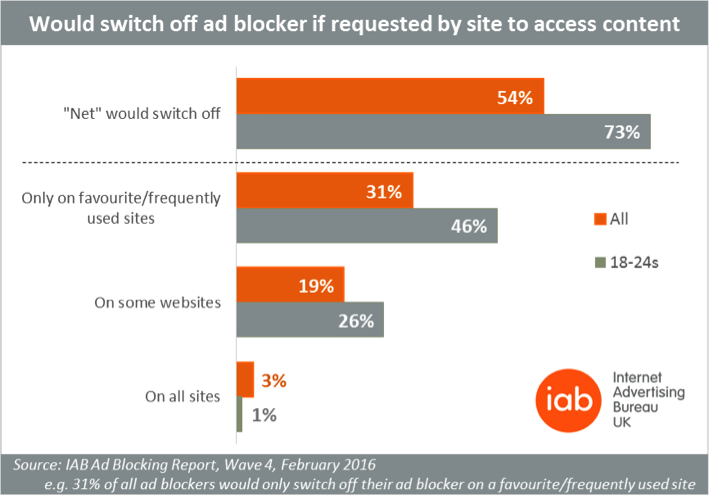
\includegraphics[width=12cm]{img/Adblockblock}
\caption{Schakelt de gebruiker een ad blocker uit?}
\label{fig: Adblockblock}
\end{figure}

\section{Gebruik maken van een paywall}
\label{sec Gebruik maken van een paywall}
Een nog hardere manier van aanpakken dan vorige methode is er voor zorgen dat niemand aan de inhoud van de betrokken website kan zonder te betalen. Er wordt geen onderscheid gemaakt of de bezoeker van de website een ad blocker gebruikt of niet, iedereen moet betalen. Het voordeel van deze methode is dat ze eenvoudig uit te voeren is, en dat ad blockers er niets kunnen tegen doen: er valt namelijk niets te blokkeren.
\\
Het grote nadeel is dat het bereik van de webpagina zeer klein is, en ze heel moeilijk verspreid kan worden over het internet. Gebruikers met een abonnement hebben dan wel toegang tot de content, ze kunnen er geen discussie over aangaan op sociale media want er is weinig kans dat vrienden en kennissen over dezelfde toegang beschikken. Ook de Nederlandstalige nieuwssite De Correspondent \footnote{\url{https://decorrespondent.nl/}} hanteert dit model, en heeft een gedeeltelijke oplossing gevonden voor de slechte bereikbaarheid. Ze laat betalende gebruikers toe om artikels te delen op sociale media met een unieke link. Via deze link is het gedeelde artikel leesbaar voor iedereen.
\\ 
Websites die dit model succesvol willen toepassen, moeten inhoud leveren van hoge kwaliteit die liefst ook uniek is. Het zal hoe dan ook moeilijk zijn om nieuwe abonnees te vinden. Een vaak gebruikte manier om toch bezoekers te lokken is om elke gebruiker een aantal gratis artikels per maand ter beschikking te stellen. Om dat te bekomen moet de gebruiker een account aanmaken. Eens dit gebeurd is, wordt het gemakkelijker om de gebruiker te verleiden tot de aankoop van een abonnement, het pad is al geëffend. De gebruiker weet ondertussen ook beter voor welke soort inhoud hij gevraagd wordt te betalen.

Er kan ook gekozen worden voor een systeem zonder abonnement maar waar per artikel betaald wordt. Blendle\footnote{\url{https://blendle.com/}} is daar een voorbeeld van.

\section{Donaties vragen}
\label{sec Donaties vragen}
Voor sommige websites is het invoeren van een abonnement niet zo evident. Eigenaars en beheerders van zo'n website kunnen in plaats van reclame te tonen, donaties vragen. Ze kunnen er voor kiezen om aan niemand reclame te tonen en aan elke bezoeker een donatie te vragen, Wikipedia werkt op deze manier. Een andere mogelijkheid is aan elke gebruiker reclame te tonen, en enkel bij gebruikers die de reclame blokkeren een donatie te vragen.
\\
\\
Het vragen van een donatie speelt in op het geweten van de gebruiker. Maar het geweten van de meeste gebruikers is snel gesust. De bezoekers die ad blockers gebruiken en bereid zijn om een donatie te doen, doen dit één of misschien twee keer, waarna hun geweten gezuiverd is. Een blijvende vervanging voor de inkomstenstroom uit reclame kan dit dus niet genoemd worden.


\section{Gesponsorde content en Affiliate marketing}
\label{sec Gesponsorde content en affiliate marketing}
Soms willen eigenaars en beheerders van websites de ad block gebruikers niet blokkeren of dwingen om te abonneren. Soms zijn donaties onvoldoende of men wil simpelweg niet bedelen. Dan kan men de manier waarop men adverteert aanpassen. Gesponsorde artikels zijn hier een voorbeeld van. Hier betaalt een derde partij om content te plaatsen op jouw platform. Een andere mogelijk is om product reviews te publiceren die gesponsord worden door de eigenaar van dat product. 
\\
In video- en beeldmateriaal kan dit op veel subtielere manieren gebeuren. Het dragen van gesponsorde kleren met merknamen op, zoals al vaker in de sportwereld gebeurt, is een eenvoudige manier om reclame in de content te verweven.
\\
Ook door middel van gesponsorde links naar andere webpagina's kan geprobeerd worden de verloren opbrengsten goed te maken.
\section{Native adverteren}
\label{sec Native adverteren}
Native adverteren is een advertentievorm die volledig past in de context en design van de website waarop hij geplaatst is. De inhoud is bedoeld voor een gerichte groep bezoekers van de website. Zo’n advertentie wordt verondersteld heel interessant en nuttig te zijn voor die specifieke doelgroep. Tot op heden ontsnapt deze vorm van reclame aan de filter van de ad blockers omdat ze niet als reclame beschouwd worden. Native adverteren is ook ontstaan als wapen tegen ad blocking. Maar haar eigen succes kan haar de das omdoen in de toekomst. Om met native adverteren een groot bereik over verschillende platformen te realiseren, is er momenteel al een ontwikkeling gaande waarin ook native advertentie URL's tot op zekere hoogte gestandaardiseerd worden. Hierdoor worden deze advertenties opnieuw vatbaar voor de gevreesde ad blockers. 
Native adverteren wordt veel beter gewaardeerd door consumenten dan de klassieke online advertenties. Uit een onderzoek van Sharethrough (\cite{ShareThrough2013}) blijkt dat consumenten 53\% vaker kijken naar native advertenties dan naar display advertenties. Daarbij zegt 32\% van de respondenten een native ad te willen delen met vrienden of familie, bij een display ad overweegt slechts 19\% dit.
Er moet ook rekening gehouden worden dat er een groot aantal gebruikers is waarvoor opzichtige aanbiedingen goed werken. Deze vervangen door enkel native te adverteren zou leiden tot een groot verlies van efficiëntie.


\chapter{Wetgeving en rechtszaken rond ad blockers}
\label{ch: Wetgevingen en rechtzaken rond ad blockers}

Volgens de Europese wetgeving is het illegaal dat websites zonder toestemming scripts draaien op apparaten van gebruikers, om te achterhalen of ze gebruik maken van ad blockers. 
In artikel 5.3 van de ePrivacy Directive staat dat het gebruik van elektronische communicatienetwerken om informatie bij de apparatuur van gebruikers op te halen of op te slaan, alleen toegestaan is onder bepaalde voorwaarden. Om aan deze voorwaarden te voldoen moet de gebruiker een helder en volledige voorlichting krijgen. En moet er expliciet om toestemming gevraagd worden. De cookiewet is een voorbeeld hiervan. Maar ook ad blocker detectiescripts vallen hieronder. De Nederlandse wetgeving vormt een uitzondering op de Europese richtlijn. Als een script geen of nauwelijks inbreuk maakt op de privacy van bezoekers, is de notificatie- en toestemmingsplicht niet van toepassing. Volgens de Autoriteit Persoonsgegevens is hier sprake van bij ad blocker detectiescripts. Nederlandse websites mogen dus wel ad blockers detecteren, hoeven gebruikers niet in te lichten over de detectie, en hoeven ook geen toestemming te vragen. 
\\
\\
Sinds mei 2011 moet volgens deze Europese wet, door de gebruiker altijd toestemming gegeven worden vooraleer een anti-ad blocker script kan draaien en je de toegang tot de pagina kan verbieden. Terwijl gewacht wordt op de toestemming van de bezoeker zou de site er kunnen voor kiezen om nog niets te tonen, maar zo worden de bezoekers die geen ad blockers gebruiken ook afgestraft. De pagina-inhoud tonen terwijl gewacht wordt op de toestemming heeft echter geen zin, want het was net de bedoeling de pagina af te schermen. Dus wordt de vraag om toestemming te geven gewoon niet gesteld. Tot nu toe, wordt ook niet gecontroleerd of deze Europese wetgeving wordt toegepast.
\\
\\
De Poolse privacy voorvechter Alexander Hanff (CEO bij Think Privacy Inc.) heeft hier omtrent in februari 2016 contact opgenomen met de Europese commissie. In april 2016 heeft hij een brief van hun ontvangen, waarin effectief wordt bevestigd dat anti-ad blocker scripts in strijd zijn met de Europese wetgeving. 
Met de ondersteuning van dit formele standpunt van de Europese Commissie, is Alexander Hanff van plan om aanklachten tegen meerdere EU-lidstaten in te dienen. Ook is hij bezig met het opzetten van een website waar een lijst bijgehouden wordt met alle websites en uitgevers die zich niet aan deze regelgeving houden. Gebruikers zullen de informatie op de site ook zelf kunnen aanvullen. Op die manier wil hij het indienen van de aanklachten vergemakkelijken.
In 2016 zijn de acties die Alexander Hanff onderneemt hieromtrent zeker verder te volgen.

\section{Rechtszaken}
\label{sec Rechtszaken}
Sinds 2014 hebben bedrijven (vooral uitgeverijen) in verschillende Europese landen een rechtszaak aangespannen tegen het bedrijf Eyeo, de ontwikkelaar van de ad blocker Adblock Plus. Volgens de uitgevers is de software van Adblock Plus in strijd met de competitie- en copyrightwetgeving. Ze eisen dat Adblock Plus de advertenties op hun sites niet meer mag blokkeren, omdat dit een ontoelaatbare ingreep is in hun diensten, die worden gefinancierd door advertenties. 
De eisen werden in het verleden steeds afgewezen door de rechtbanken. 
\\
\\
Een argument dat recent (april 2016) door een Duitse rechtbank werd gebruikt om de klacht te weerleggen was het volgende: de rechtbank wees erop dat Adblock Plus zich niet specifiek op de sites van de klagers richt, en dat gebruikers de standaardinstellingen kunnen aanpassen. De klacht van de betrokken uitgeverijen (Zeit Online en Handelsblatt) richtte zich voornamelijk op het acceptable-ads-initiatief van Adblock Plus. Hierbij kunnen sites, al dan niet tegen betaling, op de zogenaamde whitelist komen te staan als hun advertenties aan eisen voldoet die door Eyeo zijn opgesteld. De uitgeverijen noemen dit ronduit afpersingspraktijken.
Eyeo verdedigde zich met de verklaring dat 90\% van de sites die op de whitelist staan niet hoeven te betalen. De resterende 10\%, waaronder grote namen als Google en Microsoft, zou aanzienlijk meer inkomsten binnenhalen door de plaatsing op de witte lijst. 
Eerder dit jaar echter verklaarde een kleiner bedrijf tegen Financial Times 30\% van de opbrengst van de advertenties af te staan om op de whitelist te komen.
\\
Ook tegen Brave, de nieuwe browser (gelanceerd in januari 2016) die automatisch advertenties zal blokkeren wordt al actie ondernomen. Deze browser gaat zelfs nog een stap verder: Brave blokkeert niet enkel de advertenties, maar verkoopt de vrijgekomen advertentieruimte door. 55\% van de opbrengst van deze advertentieverkoop zou volgens hen worden gedeeld met de uitgevers van de websites. Maar het verwijderen van de oorspronkelijke advertenties wordt door de uitgeverijen gezien als diefstal.
In april 2016 hebben 17 Amerikaanse uitgeverijen zich gebundeld om te overwegen samen klacht in te dienen tegen Brendan Eich, de CEO en oprichter van Brave Software. Deze uitgeverijen vertegenwoordigen 1700 Amerikaanse kranten waaronder The New York Times, The Wall Street Journal, The Washington Post …
Ze dreigen een proces aan te spannen als Brave Software effectief verder gaat met hun plan om advertenties van de betrokken websites te vervangen door hun eigen advertenties. Tot een offciële klacht door NAA (Newspaper Association of America) kan nog niet overgegaan worden aangezien Brave Software deze manier van werken nog niet toepast. In hun aanklacht verwijzen ze ook naar een ouder proces uit 2003: een software genaamd Gator verving ook banner advertenties met eigen advertenties, gelijkaardig aan de praktijken van Brave. Een coalitie van uitgevers, waaronder Dow Jones en The New York Times, heeft toen het het bedrijf achter Gator aangeklaagd. Het resultaat was dat deze functie uit de software verwijderd moest worden.

%% TODO: de structuur en titel van deze hoofdstukken hangen af van je
% eigen onderzoek. Elke fase in je onderzoek kan een eigen hoofdstuk krijgen. Kies telkens een gepaste titel. ``Corpus'' is *GEEN* gepaste titel

\chapter{Conclusie}
\label{ch:conclusie}
De gevolgen van het gebruik van ad blockers zijn voor de websites die in belangrijke mate hun inkomsten halen uit reclame, goed te voelen. Het wereldwijde inkomstenverlies bedraagt miljarden dollars. Gemiddeld derven deze websites 13\% aan advertentie-inkomsten. Voor sommige sectoren loopt dit verlies zelfs op tot 70\%. Er wordt verwacht dat het gebruik van ad blockers zal blijven toenemen. Toch zien veel uitbaters van websites voorlopig de ad blockers niet als een direct gevaar voor hun voortbestaan. De reden hiervoor is het stijgend gebruik van mobiele toestellen waarop softwareoplossingen die reclame blokkeren nog niet effectief werken. De evolutie van ad blockers op mobiele toestellen wordt wel met argusogen gevolgd. 
\\
\\
Er zijn verschillende redenen voor het gebruik van ad blockers. Deze zijn o.a. : privacy, een webpagina kunnen lezen zonder afgeleid te worden door reclame, snelheid en beveiliging. Voor mobiele gebruikers komt daar nog eens het verbruik van bandbreedte bij. Advertentiebureaus beseffen dat ze het stijgend gebruik van ad blockers voor een groot stuk aan zichzelf te danken hebben. Ze proberen dan ook de advertenties aan te passen, zodat de gebruikerservaring minder negatief wordt beïnvloed. Vooral voor advertenties op mobiele toestellen is het belangrijk dat er rekening gehouden wordt met de laadtijden en de gebruikte bandbreedte. Het zijn namelijk die mobiele advertenties waar deze websites in de toekomst het meest zullen aan verdienen. Als ze er tenminste op tijd in slagen om de mobiele gebruikers niet massaal in de armen van ad blockers te jagen.
\\
\\
Naast het verbeteren van de kwaliteit van advertenties proberen beheerders nog op andere manieren het gebruik van ad blockers tegen te gaan. Dit kan variëren van de gebruiker er opmerkzaam op te maken waarom hij beter geen ad blocker gebruikt, tot ad block gebruiker de toegang te blokkeren. Doordat ad blockers constant hun software aanpassen is dit maar een tijdelijke oplossing. Er is een soort van wapenwedloop ontstaan tussen ad blockers en inhoudsleveranciers en adverteerders. Voorlopig trekken inhoudsleveranciers en adverteerders aan het kortste eind, mede doordat de wet tot nog toe aan de kant stond van de ad blockers en hun gebruikers. 
\\
\\
Vele internet-inhoudsaanbieders beseffen dat de strijd tegen advertentieblokkering moeilijk te winnen valt. Daarom zijn ze op zoek gegaan naar alternatieven om het verlies aan inkomsten te compenseren. Donaties, abonnementen, betalen per artikel, gesponsorde inhoud en native adverteren zijn methodes die hiervoor kunnen gebruikt worden.
\\
\\
Uiteindelijk moet er een evenwicht gevonden worden tussen de kost van het verstrekken van informatie, de inkomsten uit advertenties en de appreciatie van de websitegebruiker.



% TODO: Trek een duidelijke conclusie, in de vorm van een antwoord op de
% onderzoeksvra(a)g(en). Reflecteer kritisch over het resultaat. Zijn er
% zaken die nog niet duidelijk zijn? Heeft het ondezoek geleid tot nieuwe
% vragen die uitnodigen tot verder onderzoek?



\bibliographystyle{apa}
\bibliography{tin-bachproef}

%%---------- Back matter -------------------------------------------------

\listoffigures

\end{document}
